\documentclass[draft=false
              ,paper=a4
              ,twoside=false
              ,fontsize=11pt
              ,headsepline
              ,BCOR10mm
              ,DIV11
              ]{scrbook}
\usepackage[ngerman,english]{babel}
%% see http://www.tex.ac.uk/cgi-bin/texfaq2html?label=uselmfonts
\usepackage[T1]{fontenc}
\usepackage[utf8]{inputenc}
% \usepackage[latin1]{inputenc}
\usepackage{libertine}
\usepackage{pifont}
\usepackage{microtype}
\usepackage{textcomp}
\usepackage[german,refpage]{nomencl}
\usepackage{setspace}
\usepackage{makeidx}
\usepackage{listings}
\usepackage{natbib}
\usepackage[ngerman,colorlinks=true]{hyperref}
\usepackage{soul}
\usepackage{hawstyle}
\usepackage{lipsum} %% for sample text
\usepackage{scrhack} %% remove warning http://tex.stackexchange.com/questions/51867/koma-warning-about-toc
\usepackage{todonotes}
\usepackage[nomain,acronym,toc]{glossaries}
\usepackage{enumitem} % aligned description lists


\makeglossaries

\bibpunct[, ]{(}{)}{,}{a}{}{;} % correct citation format (no comma before year)

\setcounter{secnumdepth}{5} % numbering for subsubsections

\includeonly{glossar,ch01-einleitung,ch02-grundlagen,ch03-reaktive-programmierung,ch04-real-time-web,ch05-anwendung,ch06-schluss}

\graphicspath{{./logo/}{./img/}} % {./logo/} comes from hawstyle.sty (this \graphicspath overrides that one)

\lstset{literate={/}{}{0\discretionary{/}{}{/}}} % break on /
\lstset{literate={.}{}{0\discretionary{.}{}{.}}} % break on .

\lstset{breaklines=true}


%% define some colors
\colorlet{BackgroundColor}{gray!20}
\colorlet{KeywordColor}{blue}
\colorlet{CommentColor}{black!60}
%% for tables
\colorlet{HeadColor}{gray!60}
\colorlet{Color1}{blue!10}
\colorlet{Color2}{white}

%% configure colors
\HAWifprinter{
  \colorlet{BackgroundColor}{gray!20}
  \colorlet{KeywordColor}{black}
  \colorlet{CommentColor}{gray}
  % for tables
  \colorlet{HeadColor}{gray!60}
  \colorlet{Color1}{gray!40}
  \colorlet{Color2}{white}
}{}
\lstset{%
  numbers=left,
  numberstyle=\tiny,
  stepnumber=1,
  numbersep=5pt,
  basicstyle=\ttfamily\small,
  keywordstyle=\color{KeywordColor}\bfseries,
  identifierstyle=\color{black},
  commentstyle=\color{CommentColor},
  backgroundcolor=\color{BackgroundColor},
  captionpos=b,
  fontadjust=true
}
\lstset{escapeinside={(*@}{@*)}, % used to enter latex code inside listings
        morekeywords={uint32_t, int32_t}
}
\ifpdfoutput{
  \hypersetup{bookmarksopen=false,bookmarksnumbered,linktocpage}
}{}

% "define" Scala http://tex.stackexchange.com/questions/47175/scala-support-in-listings-package
\lstdefinelanguage{scala}{
  morekeywords={abstract,case,catch,class,def,%
    do,else,extends,false,final,finally,%
    for,if,implicit,import,match,mixin,%
    new,null,object,override,package,%
    private,protected,requires,return,sealed,%
    super,this,throw,trait,true,try,%
    type,val,var,while,with,yield},
  otherkeywords={=>,<-,<\%,<:,>:,\#,@},
  sensitive=true,
  morecomment=[l]{//},
  morecomment=[n]{/*}{*/},
  morestring=[b]",
  morestring=[b]',
  morestring=[b]"""
}

%% more fancy C++
\DeclareRobustCommand{\cxx}{C\raisebox{0.25ex}{{\scriptsize +\kern-0.25ex +}}}

\clubpenalty=10000
\widowpenalty=10000
\displaywidowpenalty=10000

% unknown hyphenations
\hyphenation{
}

%% recalculate text area
\typearea[current]{last}

\makeindex
\makenomenclature

\begin{document}
\selectlanguage{ngerman}
\lstset{language=Scala}

%%%%%
%% customize (see readme.pdf for supported values)
\HAWThesisProperties{Author={Till Theis}
                    ,Title={Das Play-Framework und dessen Einsatz zur Entwicklung von Real-Time-Web-Anwendungen}
                    ,EnglishTitle={The Play Framework and its Use for Developing Real-Time Web Applications}
                    ,ThesisType={Bachelorarbeit}
                    ,ExaminationType={Bachelorprüfung}
                    ,DegreeProgramme={Bachelor of Science Angewandte Informatik}
                    ,ThesisExperts={Prof.
Dr.
Friedrich Esser \and Prof.
Dr.
Zweitprüfer}
                    ,ReleaseDate={1.
Januar 2345}
                  }

%% title
\frontmatter

%% output title page
\maketitle

\onehalfspacing

%% add abstract pages
%% note: this is one command on multiple lines
\HAWAbstractPage
%% German abstract
{Schlüsselwort 1, Schlüsselwort 2}%
{Dieses Dokument \ldots}
%% English abstract
{keyword 1, keyword 2}%
{This document \ldots}

\newpage
\singlespacing

\tableofcontents
\newpage
%% enable if these lists should be shown on their own page
%%\listoftables
\listoffigures
\lstlistoflistings

%% main
\mainmatter
\onehalfspacing
%% write to the log/stdout
\typeout{===== File: chapter 1}
%% include chapter file (chapter1.tex)
%%\include{chapter1}

%%%%




%!TEX root = thesis.tex

% vgl. http://tex.stackexchange.com/questions/8946/how-to-combine-acronym-and-glossary

% \newglossaryentry{computer}{name=computer, description={is the rate of deactivation from ... and emission)}, sort=k}

% \newacronym{lvm}{LVM}{Logical Volume Manager}

% \newglossaryentry{lvm}{name=LVM, description={a Logical Volume Manager (LVM) does smth fancy}, first={Logical Volume Manager (LVM)}}



\newglossaryentry{mvc}
{
  name        = MVC,
  description = {"`[The Model-View-Controller (MVC) architecture is a] three-way factoring, whereby objects of different classes take over the operations related to the application domain (the model), the display of the application's state (the view), and the user interaction with the model and the view (the controller)."' \cite[vgl.][S.~1]{mvc}},
  first       = {Model-View-Controller (MVC)}
}


\newglossaryentry{adt}
{
  name        = algebraischer Datentyp,
  description = {ein algebraischer Datentyp ist ein aus anderen Typen zusammengesetzter Datentyp, der mittels Pattern Matching zerlegt werden kann},
}


\newglossaryentry{router}
{
  name        = Router,
  description = {der Router einer Play-Anwendung bildet URLs auf Controller-Aktionen ab},
}


\newglossaryentry{kovarianz}
{
  name        = Kovarianz,
  description = {ist ein Datentyp \lstinline|T| über einen kovarianten Typ \lstinline|A| parametrisiert, so ist \lstinline|T[B]| ein Sub-Typ von \lstinline|T[A]|, falls \lstinline|B| ein Sub-Typ von \lstinline|A| ist},
}


\newglossaryentry{nothing}
{
  name        = Nothing,
  description = {Der Scala-Typ \lstinline|Nothing| ist eine Spezialisierung jedes anderen Typs und kann deshalb jeden anderen Typ annehmen \cite[vgl.][S.~216]{programming_in_scala}},
}


\newglossaryentry{continuation}
{
  name        = Continuation,
  description = {Eine Delimited Continuation repräsentiert den Rest einer Berechnung bis zu einem bestimmten Punkt \cite[vgl.][S.~1]{continuations}},
}


\newglossaryentry{ajax}
{
  name        = Ajax,
  description = {Asynchronous JavaScript and XML (Ajax) ist eine Technik, die asynchrone Kommunikation zwischen Client und Server ermöglicht},
  first       = {Asynchronous JavaScript and XML (Ajax)}
}


\newglossaryentry{json}
{
  name        = JSON,
  description = {Mit der JavaScript Object Notation (JSON) lassen sich JavaScript-Objekte als literale notieren},
  first       = {JavaScript Object Notation (JSON)}
}


\newglossaryentry{dom}
{
  name        = DOM,
  description = {Document Object Model (JSON)},
  first       = {Document Object Model (JSON)}
}

%!TEX root = thesis.tex

\chapter{Einleitung} % (fold)
\label{cha:einleitung}

In Diesem Kapitel wird erläutert, was das Real-Time-Web ausmacht und weshalb sich das Play-Framework besonders eignet, Anwendungen dafür zu schreiben.
Es wird ein Überblick über die bisherige Entwicklung des Webs gegeben und klargestellt, womit sich diese Arbeit genau beschäftigt und womit nicht.
Anschließend wird aufgelistet, wie die weitere Struktur dieser Arbeit aussieht.


\section{Entwicklung des Webs} % (fold)
\label{sec:entwicklung_des_webs}

Nach \citealt{tavalsaari2011}~(S.~1--3) war das World Wide Web der 1990er Jahre ein Medium, bei dem einzelne Dokumente im Vordergrund standen.
Das klassische Web der ersten Hälfte des Jahrzehnts bestand aus Dokumenten mit Text, Bildern und Links.
Die zweite Hälfte machte das hybrid Web aus.
Browsertechnologien, wie Javascript und CSS, sowie Plugins wie Flash und QuickTime wurden entwickelt und erweiterten die statischen Dokumente um interaktive Elemente.

In den 2000ern verbreitete sich das dynamische Senden und Anfordern von Daten unter dem Namen Ajax (Asynchronous JavaScript and XML).
Gegen Ende des Jahrzehnts wurden die vorhandenen Technologien genutzt, um ganze Anwendungen damit zu schreiben, wie z.~B. Facebook oder Twitter.

% section entwicklung_des_webs (end)


\section{Real-Time-Web} % (fold)
\label{sec:real-time-web}

Eine Real-Time-Web-Anwendung ist eine Web-Anwendung, die automatisch neue Daten an den Client sendet, sobald diese dem Server bekannt werden.
Dies unterscheidet sich vom klassischen Pull-Prinzip, in dem nur der Client per Anfrage eine neue Seite beim Server anfordern kann.
Bei Real-Time-Events ist es stattdessen notwendig, dass der Server mittels Push-Prinzip neue Informationen an den Client sendet \cite[vgl.][S.~1]{bozdag2007}.
Facebook beispielsweise zeigt neue Statusmeldungen von Freunden an, ohne dass manuell die Seite neu geladen werden muss.

% section real-time-web (end)


\section{Motivation} % (fold)
\label{sec:motivation}

Wenn man die in Kap.~\ref{sec:entwicklung_des_webs} beschriebene Entwicklung des Webs betrachtet, knüpft das Real-Time-Web genau daran an.
Der Nachrichtenverkehr verläuft nicht mehr nur vom Client zum Server, sondern auch in umgekehrter Richtung vom Server zum Client.
Das Play-Framework besitzt Werkzeuge, mit dieser Art der Kommunikation umzugehen~\cite[vgl.][S.~5]{drobi2012}.

% section motivation (end)


\section{Themenabgrenzung} % (fold)
\label{sec:themenabgrenzung}

Diese Arbeit beschäftigt sich in erster Linie mit der Architektur und den Grundlagen des Play-Frameworks und den Teilen, die zur Entwicklung von Real-Time-Web-Anwendungen benötigt werden.
Einige Themenbereiche, die dafür nicht elementar sind, wie z.~B. Datenbanken, werden nicht behandelt.
Des Weiteren wird vorausgesetzt, dass der Leser bereits mit den Grundtechnologien der Web-Entwicklung, wie HTML, CSS und Javascript vertraut ist.

% section themenabgrenzung (end)


\section{Ziel} % (fold)
\label{sec:ziel}

Das Ziel dieser Arbeit ist es, das Play-Framework in Scala zu analysieren und dessen Grundlagen zu erklären, um schließlich seine Werkzeuge zur Entwicklung von Real-Time-Web-Anwendungen zu erforschen.
Auf Basis dieser Erkenntnisse wird anschließend eine Beispielanwendung analysiert und eine eigene Anwendung geschrieben, die das Real-Time-Prinzip ausnutzt.

% section ziel (end)


\section{Struktur} % (fold)
\label{sec:struktur}

% section struktur (end)


% chapter einleitung (end)
%!TEX root = thesis.tex

\chapter{Grundlagen} % (fold)
\label{cha:grundlagen}

In diesem Kapitel werden die grundlegenden Techniken zur Webseiten-Entwicklung mit dem Play-Framework vorgestellt.
Dabei wird notwendiges Hintergrundwissen bereitgestellt und erklärt, welche Werkzeuge benötigt werden.
Schließlich werden durch die Entwicklung einer kleinen Anwendung die einzelnen Komponenten erklärt.
Es werden hierbei in erster Linie die Komponenten vorgestellt, die für die Entwicklung von Real-Time-Web-Anwendungen unbedingt notwendig sind.


\section{Vorbereitung} % (fold)
\label{sec:vorbereitung}

Bevor auf die eigentliche Arbeit mit dem Play-Framework eingegangen wird, müssen einige vorbereitende Dinge erklärt werden.
In diesem Abschnitt geht es darum, wie die Entwicklungsumgebung aufgesetzt wird, mit welcher Version der eingesetzten Software gearbeitet wird und wie sich das Play-Framework installieren lässt.

\subsection{Entwicklungsumgebung} % (fold)
\label{sub:entwicklungsumgebung}

Zum Anlegen von Play-Projekten und Steuern des Web-Servers wird eine Kommandozeile, wie die Eingabeaufforderung unter Windows oder dem Terminal und Mac OS~X benötigt.
Zum Programmieren kann entweder ein einfacher Text-Editor, oder auch eine IDE verwendet werden.
Für die einzelnen Programme können teilweise Plugins heruntergeladen werden, die beispielsweise Code Completion oder Syntax Highlighting für Play-spezifische Funktionalitäten bereitstellen.

Für \textbf{Eclipse} kann die Scala IDE von \citealt{scala_ide} heruntergeladen werden.
Diese IDE ist für die Entwicklung von Scala-Anwendungen mit Eclipse notwendig.
Für die Scala IDE existiert außerdem ein Plugin für das Play-Framework.
Eine genaue Installationsanleitung dafür ist unter \citealt{scala_ide_play_plugin} zu finden.
Um ein Play-Projekt in Eclipse zu bearbeiten, muss dafür nach dem Anlegen des Projekts auf der Kommandozeile ein Eclipse-Projekt exportiert werden.
Dazu muss in der Play-Konsole des Projekts der Befehl \lstinline|eclipse| ausgeführt werden.
Dieser Befehl muss jedes Mal ausgeführt werden, wenn die Konfigurationsdateien geändert werden.
Anschließend kann der Ordner des Play-Projekts als Eclipse-Projekt importiert und geöffnet werden.

Beim Exportieren eines \textbf{IntelliJ IDEA}-Projekts verhält es sich ähnlich, wie im Falle von Eclipse.
Der einzige Unterschied ist, dass der Befehel \lstinline|idea| verwendet werden muss, um ein IntelliJ IDEA-Projekt zu erstellen.
Für Text-Editoren, wie z.B. \textbf{VIM}, \textbf{Emacs} oder \textbf{Sublime Text} ist prinzipiell kein Plugin nötig.
Falls aber ein Plugin für den verwendeten Editor existiert, kann es natürlich installiert werden.
Weitere Informationen zu diesen und \textbf{anderen Entwicklungsumgebungen} sind in der offiziellen Dokumentation zu finden \cite[vgl.][]{ide}.

% subsection entwicklungsumgebung (end)


\subsection{Software-Version} % (fold)
\label{sub:software_version}

Zum Zeitpunkt dieser Arbeit ist die aktuellste stabile Version des Play-Frameworks die Version 2.2.0.
Diese Version wird in allen Beispielen und der eigenen entwickelten Anwendung verwendet.
Für den Einsatz des Frameworks wird das JDK in Version 6 oder 7 benötigt.
Der Autor arbeitet mit dem JDK~7 unter Mac OS~X.
Die aktuell verwendete Scala-Version ist 2.10.2, diese ist unabhängig von der systemweit installierten Version und wird beim Anlegen eines Play-Projekts für das jeweilige Projekt installiert.

% subsection software_version (end)


\subsection{Installation} % (fold)
\label{sub:installation}

Zum Installieren von Play kann eine vorkompilierte Version der Software von der offiziellen Website unter \cite{play_download} heruntergeladen werden.
Nach dem Entpacken der heruntergeladenen Datei kann das Programm namens \lstinline|play|, das sich im entpackten Ordner befindet, auf der Kommandozeile verwendet werden.
Um für die Verwendung des Programms nicht immer den absoluten Pfad angeben zu müssen, kann der Pfad zum entpackten Ordner in die Systemumgebungsvariable PATH eingetragen werden.

Unter \textbf{Mac OS~X} muss dazu auf der Kommandozeile folgender Befehl ausgeführt werden: \lstinline|export PATH=$PATH:<Pfad zum entpackten Ordner>|.
Ein konkretes Beispiel könnte so aussehen: \lstinline|export PATH=$PATH:~/Downloads/play-2.1.3|.
Damit sich der Ordner auch nach dem Schließen des Terminals noch in der \lstinline|PATH|-Variable befindet, sollte der obige Befehl zusätzlich in die \lstinline|~/.profile|-Datei oder in die Konfigurationsdatei der verwendeten Shell eingetragen werden.
Falls diese Datei nicht existiert, muss sie vorher angelegt werden.

Unter \textbf{Windows} muss dazu in der Eingabeaufforderung folgender Befehl ausgeführt werden: \lstinline|setx PATH "%PATH%;c:\path\to\play" /m|, wobei \lstinline|c:\path\to\play| durch den tatsächlichen Pfad zu ersetzen ist \cite[vgl.][S.~9]{play_for_scala}.

% subsection installation (end)


% section vorbereitung (end)


\section{Beispielanwendung: Sammeln von Altersstatistiken} % (fold)
\label{sec:beispielanwendung}

Um die Techniken zur Entwicklung von statischen Web-Anwendungen zu demonstrieren, soll im Folgenden eine kleine Anwendung entwickelt werden.
Diese Anwendung fragt ihre Benutzer, wie alt sie sind und bildet die gesammelten Information als Diagramm ab.
Anhand dieser Anwendung soll die Entwicklung mit Models, Views und Controllern erklärt werden.
Bevor mit der Implementierung gestartet werden kann, muss allerdings die die Grundarchitektur des Frameworks erklärt werden.


\subsection{Architektur} % (fold)
\label{sub:architektur}

Auf der untersten Ebene existiert ein Web-Server, der mit dem Framework ausgeliefert wird.
Die Anfragen, die der Web-Server empfängt werden an Play weitergeleitet und schließlich von der Anwendung verarbeitet.
Nach der Verarbeitung wird eine Antwort generiert und schließlich als HTTP-Antwort versendet.
Der Anwendungscode einer Play-Applikation ist nach der Model-View-Controller-Architektur (MVC) aufgebaut.

Models beinhalten die Anwendungslogik der Applikation.
Views stellen Informationen der Models i.~d.~R. als HTML-Seiten dar.
Controller bilden eingehende HTTP-Anfragen mit Hilfe von Models und Views auf HTTP-Antworten ab.
Controller empfangen HTTP-Anfragen, berechnen mit Hilfe der Models eine Antwort, lassen diese von einer View übersetzen, um das Ergebnis der View schließlich als HTTP-Antwort zurückzusenden \cite[vgl.][S.~45--48]{play_for_scala}.

Ruft ein(e) WebseitenbesucherIn beispielsweise ein Nutzerprofil auf, so generiert der Web-Browser eine HTTP-Anfrage, die an den von Play verwendeten Web-Server gesendet wird.
Das Play-Framework ermittelt den zuständigen Controller für die Anfrage und übergibt ihm diese.
Der Controller sucht mit Hilfe der Anwendungslogik den passenden Nutzer (z.~B. aus der Datenbank) heraus und übergibt dieses Nutzer-Model an die passende View.
Die View bereitet die im Nutzer-Model gekapselten Informationen als HTML-Seite auf.
Anschließend gibt der Controller diese HTML-Darstellung des Nutzerprofils zurück, was vom Web-Server dann an den Web-Browser gesendet und schließlich dem/der Webseitenbesucher(in) angezeigt wird.

% subsection architektur (end)


\subsection{Erstellen einer Anwendung} % (fold)
\label{sub:erstellen_einer_anwendung}

Um eine neue Anwendung mit Play zu erstellen, muss auf der Kommandozeile in den Ordner navigiert werden, in dem das Projekt erstellt werden soll.
Anschließend kann mit \lstinline[language=sh]|play new <project name>| ein neues Projekt angelegt werden.
In diesem Fall ist der Projektname \lstinline|age_statistics_http|.
Im startenden Assistenten wählt man die Hauptprogrammiersprache aus (Java oder Scala), in diesem Fall Scala.
Daraufhin wird im aktuellen Verzeichnis ein neuer Ordner mit dem vorher angegebenen Namen \lstinline|age_statistics| angelegt \cite[vgl.][S.~10]{play_for_scala}.
Die darin vorzufindende Verzeichnisstruktur wird im nächsten Unterabschnitt beschrieben.

% subsection erstellen_einer_anwendung (end)


\subsection{Verzeichnisstruktur} % (fold)
\label{sub:verzeichnisstruktur}

Die Verzeichnisstruktur einer Play-Anwendung ist immer gleich.
An dieser Stelle werden nur die Ordner vorgestellt, die für das Verständnis dieser Arbeit wichtig sind.
Diese Ordner sind folgende \cite[vgl.][]{play_verzeichnisstruktur}:

\begin{description}[leftmargin=!,labelwidth=\widthof{\bfseries app/controllers/}]
  \item[app/] ausführbare Komponenten
  \item[app/controllers/] Controller-Komponenten
  \item[app/models/] Model-Komponenten
  \item[app/views/] View-Komponenten
  \item[conf/] Konfigurationsdateien
  \item[public/] öffentliche statische Dateien (JS, CSS, Bilder)
\end{description}

% subsection verzeichnisstruktur (end)


\subsection{Starten einer Anwendung} % (fold)
\label{sub:starten_einer_anwendung}

Um die neu erstellte Anwendung zu starten, muss sie erst kompiliert werden.
Das geschieht ebenfalls mit Hilfe des \lstinline|play|-Befehls.
Mit dem Aufruf von \lstinline|play| gelangt man in die Play-Konsole.
Von dort aus kann mit \lstinline|compile| der Source-Code kompiliert und anschließend mit \lstinline|run| ausgeführt werden.
Der Aufruf von \lstinline|compile| ist allerdings optional.
Falls noch nicht kompilierte Änderungen existieren, werden diese beim Aufruf von \lstinline|run| automatisch kompiliert, sobald die Website aufgerufen wird \cite[vgl.][]{play_compile}.

Jede neue Play-Anwendung ist bereits eine lauffähige Website.
Diese kann nach dem Starten unter der URL \url{http://localhost:9000/} abgerufen werden (siehe Abb.~\ref{fig:anwendung_nach_erstellung}).
Um die Anwendung bei Dateiänderungen automatisch neu kompilieren zu lassen, ohne sie erst im Browser aufrufen zu müssen, kann in der Play-Konsole statt \lstinline|run| \lstinline|~run| ausgeführt werden \cite[vgl.][S.~12]{play_for_scala}.

\begin{figure}
\centering
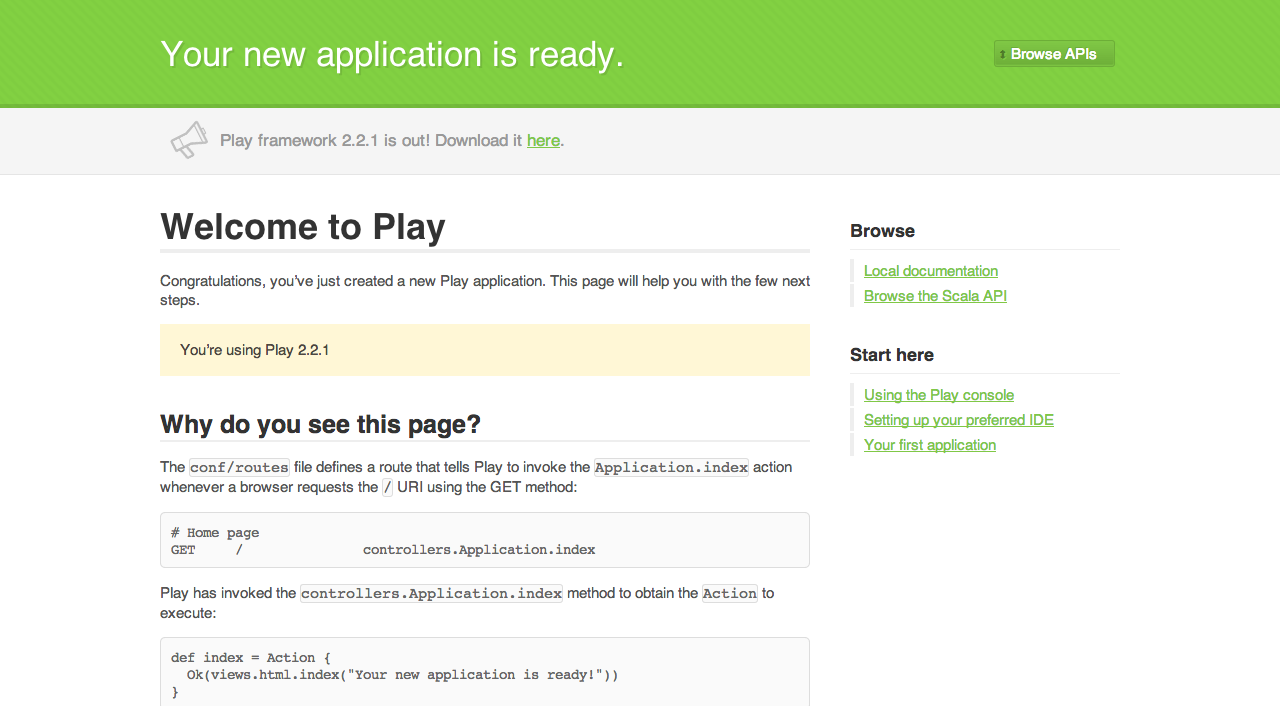
\includegraphics[width=\textwidth]{hello_world.png}
\caption{Eine neu erstellte Play-Anwendung}
\label{fig:anwendung_nach_erstellung}
\end{figure}

% subsection starten_einer_anwendung (end)


\subsection{Routing} % (fold)
\label{sub:routing}

Wenn die Website von jemandem aufgerufen wird, soll eine bestimmte Controller-Aktion ausgeführt werden.
Damit Play weiß, welche Controller-Aktion für die aufgerufene URL ausgeführt werden soll, muss dies in der \lstinline|routes|-Datei definiert werden.
Diese Datei befindet sich unter \lstinline|conf/routes| und besitzt nach der Erstellung einer Anwendung bereits zwei Einträge (vgl. Listing~\ref{lst:die_routes_datei}).
An dieser Stelle ist allerdings nur der erste Eintrag interessant.

\begin{lstlisting}[caption=Die routes-Datei, label=lst:die_routes_datei]
  GET    /    controllers.Application.index
\end{lstlisting}

Dieser Eintrag bedeutet, dass HTTP-Anfragen der Methode \lstinline|GET| der URL \lstinline|/| auf die Controller-Aktion \lstinline|index| des Controllers \lstinline[breaklines=true]|controllers.Application| abgebildet werden.
Neben \lstinline|GET| gibt es noch \lstinline|POST|, \lstinline|PUT|, \lstinline|DELETE| und \lstinline|HEAD|.
Die am Häufigsten verwendeten HTTP-Methoden sind \lstinline|GET|, \lstinline|POST|, \lstinline|PUT| und \lstinline|DELETE|, um Daten abzufragen, zu bearbeiten, zu erstellen und zu löschen \cite[vgl.][S.~7]{play_for_scala}.
Der Pfad \lstinline|/| steht für die URL \url{http://localhost:9000/}.
Es sind auch längere Pfade, wie z.~B. \lstinline|/animals/cat| möglich, davon wird in diesem Beispiel allerdings nicht Gebrauch gemacht.
Die Controller-Aktion \lstinline|controllers.Application.index|, auf die der Routing-Eintrag zeigt, ist bereits implementiert.
Diese wird in Unterabschnitt~\ref{sub:controller} allerdings durch eine eigene Implementierung ersetzt.

% subsection routing (end)


\subsection{Model} % (fold)
\label{sub:model}

Bevor die Anwendung Daten anzeigen kann, muss eine Datenstruktur für die Altersstatistiken entworfen werden.
Für diese Statistik sollen nur die Alterszahlen und die Personenzahl des jeweiligen Alters gesammelt werden.
Dafür eignet sich eine \lstinline|Map[Int, Int]|, wobei die Schlüssel das Alter sind und die Werte dazu die Anzahl an Personen, die dieses Alter haben.
Um den Code verständlicher zu machen, wird ein Typ-Alias mit dem Namen \lstinline|AgeStatistics| eingeführt.
Dies wird in der Datei \lstinline[language=sh]|app/models/package.scala| durchgeführt und hat den in Listing~\ref{lst:der_agestatistics_typ_alias} gezeigten Inhalt.
Die Verwendung eines \lstinline|package object|s ist nötig, um den Typ-Alias paket-weit einzurichten \cite[vgl.][]{package_objects}.

\begin{lstlisting}[caption=Der AgeStatistics-Typ-Alias, label=lst:der_agestatistics_typ_alias]
package object models {
  type AgeStatistics = Map[Int, Int]
}
\end{lstlisting}

Um die Verwendung noch komfortabler zu machen, wird in \lstinline|app/models/AgeStatistics.scala| ein Objekt mit Konstruktormethoden erstellt, wie in Listing~\ref{lst:das_agestatistics_hilfsobjekt} zu sehen.
Es wird eine \lstinline|apply|-Methode zur Verfügung gestellt, sodass die Werte der Statistik direkt übergeben werden können, wie z.~B. \lstinline|AgeStatistics(6 -> 1, 10 -> 2)|.
Dadurch, dass \lstinline|AgeStatistics.empty| für undefinierte Schlüssel einen Standardwert von null~(0) zurückgibt, können auch unbekannte Alterseinträge abgefragt werden, ohne dass ein Fehler auftritt.

\begin{lstlisting}[caption=Das AgeStatistics-Hilfsobjekt, label=lst:das_agestatistics_hilfsobjekt]
object AgeStatistics {
  def apply(statistics: (Int, Int)*): AgeStatistics =
    empty ++ Map(statistics: _*)
  val empty: AgeStatistics = Map.empty.withDefaultValue(0)
  val sample: AgeStatistics = apply( 6 -> 1 /* , ... */ )
}
\end{lstlisting}

% subsection model (end)


\subsection{Controller} % (fold)
\label{sub:controller}

\begin{sloppypar} % larger word spacing so that \lstinline will not go out of line margin
Nachdem im Router definiert wurde, welche URLs auf welche Controller-Aktionen abgebildet werden sollen, werden die betroffenen Controller-Aktionen nun implementiert.
Die zuvor genannte Aktion \lstinline|controllers.Application.index| befindet sich in der Datei \lstinline|app/controllers/Application.scala|.
Die Standardimplementierung wird wie in Listing~\ref{lst:application_controller_mit_index_aktion} zu sehen, umdefiniert.
\end{sloppypar}

\begin{lstlisting}[caption=Der Application-Controller mit index-Aktion, label=lst:application_controller_mit_index_aktion]
object Application extends Controller {
  def index = Action {
    Ok(views.html.index(AgeStatistics.sample))
  }
}
\end{lstlisting}

Controller sind Objekte, die von \lstinline|Controller| erben und Aktionen definieren.
Aktionen, die beim Aufruf einer URL ausgeführt werden sollen, sind Controller-Objekt-Methoden mit dem Rückgabetyp \lstinline|Action|.
Eine Aktion, bzw. \lstinline|Action| ist eine Funktion von einer HTTP-Anfrage nach einer HTTP-Antwort.
In der obigen Form wird die HTTP-Anfrage ignoriert, es können aber auch \lstinline|Action|s mit explizitem oder implizitem Request-Parameter erstellt werden \cite[vgl.][]{play_controllers}.
Dies ist z.~B. dann notwendig, wenn Formulare verarbeitet werden sollen, was in Unterabschnitt~\ref{ssub:formularverarbeitung_im_controller}~(\nameref{ssub:formularverarbeitung_im_controller}) zu sehen ist.

Um eine HTTP-Antwort zu generieren, stellt das Objekt \lstinline|play.api.mvc.Results|, von dem \lstinline|play.api.mvc.Controller| erbt, mehrere Konstruktoren zur Verfügung.
Der in Listing~\ref{lst:application_controller_mit_index_aktion} verwendete Konstruktor \lstinline|Ok| erstellt eine HTTP-Antwort mit dem Status-Code \lstinline|200 OK|.
Der Inhalt dieser Antwort ist das Ergebnis der View \lstinline|views.html.index|, worauf im folgenden Unterabschnitt näher eingegangen wird.
Neben \lstinline|Ok| gibt es u.~a. noch \lstinline|BadRequest| für fehlerhafte Anfragen (z.~B. unvollständiges Formular) und \lstinline|Redirect|, um eine Seitenweiterleitung auf eine angegebene URL durchzuführen \cite[vgl.][]{play_controllers}.

% subsection controller (end)


\subsection{View} % (fold)
\label{sub:view}

Im vorigen Unterabschnitt wurde gezeigt, wie mittels \lstinline|Ok(views.html.index(ageStatistics))| eine View gerendert und als HTTP-Antwort verschickt werden kann.
Das dazugehörige View-Template befindet sich unter \lstinline|app/views/index.scala.html|.
Bevor die Implementierung dieses Templates gezeigt wird, soll an einem einfacheren Beispiel verdeutlicht werden, wie View-Templates geschrieben werden.

\subsubsection{Views in Play} % (fold)
\label{ssub:views_in_play}

\begin{lstlisting}[caption=Ein einfaches View-Template, label=lst:ein_einfaches_view_template]
@(title: String)

@import scala.math.pow

<!doctype html>
<meta charset="utf-8">
<title>@title</title>
<p>4^3 = @{pow(4, 3)}</p>
@Html("<p>This is a simple view template.</p>")
\end{lstlisting}

Anhand des in Listing~\ref{lst:ein_einfaches_view_template} gezeigten Codes sollen Struktur und Verwendung von View-Templates in Play veranschaulicht werden.
View-Templates bestehen aus Scala- und HTML-Code und verhalten sich wie Funktionen, die HTML-Code generieren.
Am Anfang eines Templates steht die Parameterliste, worüber die anzuzeigenden Daten übergeben werden.
Nach der Parameterliste können Pakete importiert werden.
Das \lstinline|@|-Symbol führt einen Scala-Ausdruck an, der in geschweifte Klammern (\lstinline|{}|) eingeschlossen werden kann \cite[vgl.][]{play_templates}.

Neben den Template-Parametern und den importierten Paketen können sog. Helper verwendet werden.
Helper sind in Funktionen ausgelagerter Template-Code \cite[vgl.][S.~179]{play_for_scala}.
Play kodiert aus Sicherheitsgründen Scala-Strings automatisch so, dass dadurch kein HTML-Code generiert werden kann.
Um dies zu verhindern, kann der \lstinline|Html|-Helper verwendet werden, wie in der letzten Zeile von Listing~\ref{lst:ein_einfaches_view_template} zu erkennen.
Dieser Helper nimmt als Argument einen String und fügt diesen unverändert an der Stelle des Aufrufs im Template ein \cite[vgl.][]{play_templates}.

% subsubsection views_in_play (end)

\subsubsection{Altersstatistiken-View} % (fold)
\label{ssub:altersstatistiken_view}

Das eigentliche View-Template unter \lstinline|app/views/index.scala.html| ist etwas umfangreicher.
Das Zeichnen des Diagramms erfolgt Client-seitig via JS und ist in \lstinline|public/javascripts/main.js| ausgelagert.
Dieses Script wird wie auch alle anderen Dateien im \lstinline|public/|-Ordner via \lstinline|@routes.Assets.at("javascripts/main.js")| adressiert \cite[vgl.][S.~111]{play_for_scala}.
Das gesamte Template hat den in Listing~\ref{lst:das_view_template} vereinfacht dargestellten Inhalt.

\begin{lstlisting}[language=html,caption=Das View-Template, label=lst:das_view_template]
@(statistics: AgeStatistics)
<script src="@routes.Assets.at("javascripts/main.js")"></script>
<div id="ageChart"><svg></svg></div>
<script>
  var statistics = @Html(Json.toJson(statistics.map {
    case (k, v) => (k.toString, v)
  }).toString);
  makeAgeStatisticsChart("#ageChart svg", statistics);
</script>
\end{lstlisting}

\lstinline|makeAgeStatisticsChart| erwartet neben dem CSS-Selector, der das Diagramm-Element identifiziert, die Altersstatistiken, die auf Server-Seite als \lstinline|Map| vorliegen.
Diese werden auf der JS-Seite als Objekt erwartet, weil JS keine \lstinline|Map|s kennt, aber Objekte eine ähnliche Funktionalität bieten.
Weil JS-Objekte die Schlüsselwerte als \lstinline|String| erwarten, müssen die Schlüssel serverseitig erst in \lstinline|String|s konvertiert werden.
Anschließend kann mittels \lstinline|Json.toJson| die \lstinline|Map| in ein JS-Objekt konvertiert und mit \lstinline|toString| und \lstinline|Html| in das Template eingefügt werden.
Das \lstinline|play.api.libs.json|-Paket enthält verschiedene Werkzeuge, um Scala-Werte in eine JS-kompatible Darstellung zu konvertieren und umgekehrt.
\lstinline|Json.toJson| ist ein besonders einfacher Weg diese Konvertierung durchzuführen und funktioniert ohne weiteres Zu-Tun für unterschiedliche Scala-Typen, darunter auch \lstinline|Map[String, Int]| \cite[vgl.][S.~214--215]{play_for_scala}.
Wenn die \lstinline|statistics|-Variable serverseitig \lstinline|Map(51 -> 3, 16 -> 5, 10 -> 2)| enthält, so wird dies für die Client-Seite in \lstinline|{"51":3,"16":5,"10":2}| konvertiert.
Aus diesen konvertierten Daten wird dann das Diagramm erstellt, das in Abb.~\ref{fig:die_altersstatistiken_view} zu sehen ist.

\begin{figure}
\centering
\includegraphics[width=\textwidth]{age_statistics_only.png}
\caption{Die Altersstatistiken-View}
\label{fig:die_altersstatistiken_view}
\end{figure}

% subsubsection altersstatistiken_view (end)

% subsection view (end)


\subsection{Sammeln der Statistiken} % (fold)
\label{sub:sammeln_der_statistiken}

Die Nutzer sollen die Möglichkeit erhalten, der Website mitzuteilen, wie alt sie sind, um in die Statistik einzugehen.
Um das Beispiel einfach zu halten, soll nicht geprüft werden, ob jemand bereits sein Alter angegeben hat.
Um die Anwendung um Nutzer-Interaktion zu erweitern, müssen View, Routen-Datei und Controller erweitert werden.

\subsubsection{Formular in der View} % (fold)
\label{ssub:formular_in_der_view}

Um die Nutzer nach ihrem Alter zu fragen, benötig es erst einmal ein Formular, über das sie ihre Daten angeben können.
Dieses Formular ist der View schnell mit einigen Zeilen HTML hinzugefügt, wie in Listing~\ref{lst:das_view_template_mit_formular} zu sehen.
Der Einfachheit halber werden nur Altersangaben zwischen einem und 99 Jahren akzeptiert.

\begin{lstlisting}[language=html, caption=Das View-Template mit Formular, label=lst:das_view_template_mit_formular]
<form method="post" action="@routes.Application.input">
  <fieldset>
    <legend>Your Age</legend>
    <div>
      <label for="ageInput">How Old Are You?</label>
      <input type="number" min="1" max="99" id="ageInput" name="age" placeholder="Enter Age">
    </div>
    <button type="submit">Submit</button>
  </fieldset>
</form>
\end{lstlisting}

Der im obigen Listing zu sehende Code \lstinline|@routes.Application.input| ist ein Beispiel von sog. Reverse Routing.
Dabei wird die URL für einen Routen-Eintrag in der \lstinline|routes|-Datei berechnet und muss deshalb bei Änderungen nicht auch in der View geändert werden \cite[vgl.][S.~98--100]{play_for_scala}.
In diesem Fall wird die URL für die Controller-\lstinline|Action|, die für die Formularverarbeitung zuständig ist von einem Helper generiert.
Die hier verwendete Routing-Eintrag wird im folgenden Unterabschnitt angelegt.

% subsubsection formular_in_der_view (end)

\subsubsection{Eintrag in der Routen-Datei} % (fold)
\label{ssub:eintrag_in_der_routen_datei}

Wenn dieses Formular abgesendet wird, wird nicht wie zuvor ein \lstinline|GET|-Request an den Server gesendet, sondern ein \lstinline|POST|-Request, wie im \lstinline|method|-Attribut des \lstinline|form|-Tags angegeben.
In der \lstinline|conf/routes|-Datei muss deshalb ein neuer Eintrag hinzugefügt werden, der \lstinline|POST|-Requests abdeckt und an den Controller weiterleitet, wie in Listing~\ref{lst:die_routen_eintrag_fuer_formulareingaben} zu sehen.

\begin{lstlisting}[caption=Die Routen-Eintrag für Formulareingaben, label=lst:die_routen_eintrag_fuer_formulareingaben]
POST    /    controllers.Application.input
\end{lstlisting}

% subsubsection eintrag_in_der_routen_datei (end)

\subsubsection{Dynamische Statistiken und Formularverarbeitung im Controller} % (fold)
\label{ssub:formularverarbeitung_im_controller}

Damit die Statistiken aktualisiert werden können, wird der Einfachheit halber direkt im \lstinline|Application|-Controller mit \lstinline|var ageStatistics = AgeStatistics.empty| eine Variable eingeführt, die den aktuellen Wert der Statistiken enthält.
Es wäre auch möglich, ein Model anzulegen, welches die aktuelle Statistik hält, doch weil in diesem Beispiel nur der \lstinline|Application|-Controller auf die Statistik zugreift, ist es auch möglich, die aktuelle Statistik direkt im Controller zu hinterlegen.
Die Controller-\lstinline|Action|s arbeiten nun nur noch mit diesem Wert, anstatt mit \lstinline|AgeStatistics.sample|, wie es vorher der Fall war.

Der Routen-Eintrag für das Formular definiert, dass \lstinline|POST|-Requests auf den Pfad \lstinline|/| an die \lstinline|input|-Action des \lstinline|constrollers.Application|-Controllers weitergeleitet werden sollen.
Diese Action wird definiert, wie in Listing~\ref{lst:formularverarbeitung_im_controller} zu sehen.

\begin{lstlisting}[caption=Formularverarbeitung im Controller, label=lst:formularverarbeitung_im_controller]
val ageForm = Form("age" -> number(1, 99))

def input = Action { implicit request =>
  ageForm.bindFromRequest.fold(
    invalidForm => BadRequest(invalidForm.errorsAsJson.toString),
    { case (age) =>
      ageStatistics =
        ageStatistics.updated(age, ageStatistics(age) + 1)
      Redirect(routes.Application.index)
    }
  )
}
\end{lstlisting}

Das obige Listing beginnt mit der Definition der Server-seitigen Formulardarstellung.
\lstinline|ageForm| enthält die Formulardefinition für die Altersangabe.
\lstinline|play.api.data.Form.apply| erstellt aus einem \lstinline|play.api.data.Mapping| ein \lstinline|play.api.data.Form|-Objekt.
Ein \lstinline|Mapping| bildet ein oder mehrere Formularfelder auf einen Wert mit assoziiertem Datentyp ab.
Das \lstinline|play.api.data.Forms|-Hilfsobjekt enthält u.~a. die Methode \lstinline|tuple|, die aus Paaren von Formularfeldname und \lstinline|Mapping| ein einziges \lstinline|Mapping|-Objekt erstellt.
\lstinline|tuple("name" -> text, "age" -> number)| würde ein \lstinline|Mapping| für zwei Formularfelder erstellen, das beide Werte auf ein Tupel abbildet.
\lstinline|text| und \lstinline|number| sind vordefinierte \lstinline|Mapping|s des \lstinline|Forms|-Hilfsobjekts, die Zeichenketten, bzw. Zahlen erwarten \cite[vgl.][S~174--175]{play_for_scala}.
Für den Fall dass nur ein Formularfeld erwartet wird, gibt es eine weitere Variante von \lstinline|Form.apply|, die einen Formularfeldnamen und ein \lstinline|Mapping| erwartet, welche in Listing~\ref{lst:formularverarbeitung_im_controller} verwendet wird.
Dem verwendeten \lstinline|number|-Mapping werden außerdem noch Mindest- und Höchstwert mitgeteilt, damit nur glaubwürdige Werte in die Statistik gelangen.

Die \lstinline|input|-Action benötigt einen \lstinline|Request|-Parameter, um die Formulardaten lesen zu können.
\lstinline|ageForm.bindFromRequest| füllt die Server-seitige Darstellung des Formulars über den impliziten \lstinline|Request|-Parameter mit Daten, womit mittels der \lstinline|fold|-Methode dann weitergearbeitet werden kann \cite[vgl.][S.~179]{play_for_scala}.
\lstinline|fold| nimmt als Argumente zwei Funktionen.
Die erste Funktion wird ausgeführt, wenn die Formulardaten nicht auf die interne Formulardarstellung abgebildet werden konnten.
Die zweite Funktion wird ausgeführt, wenn es keine Fehler gab, dann kann mit den übergebenen Formulardaten weitergearbeitet werden \cite[vgl.][S.~176]{play_for_scala}.

In der \lstinline|input|-Action wird im Fehlerfall eine Fehlermeldung angezeigt, die zum Zwecke dieses Beispiels nur im \gls{json}-Format vorliegt, die von Play automatisch generiert wird.
Der Fehlerfall kann eintreten, obwohl in der View Minimum und Maximum des Altersfeldes angegeben sind, wenn z.~B. der Nutzer die Prüfung aus dem ausgelieferten HTML-Code entfernt.
Tritt kein Fehler auf, so werden die Altersstatistiken aktualisiert und eine Weiterleitung auf die \lstinline|index|-Action ausgelöst.
Dadurch landet der Nutzer/die Nutzerin nach Versendung des Formulars wieder auf der Hauptseite und sieht die aktualisierte Statistik.
Die finale Version der Website ist in Abb.~\ref{fig:die_altersstatistiken_view_mit_formular} zu sehen.

\begin{figure}
\centering
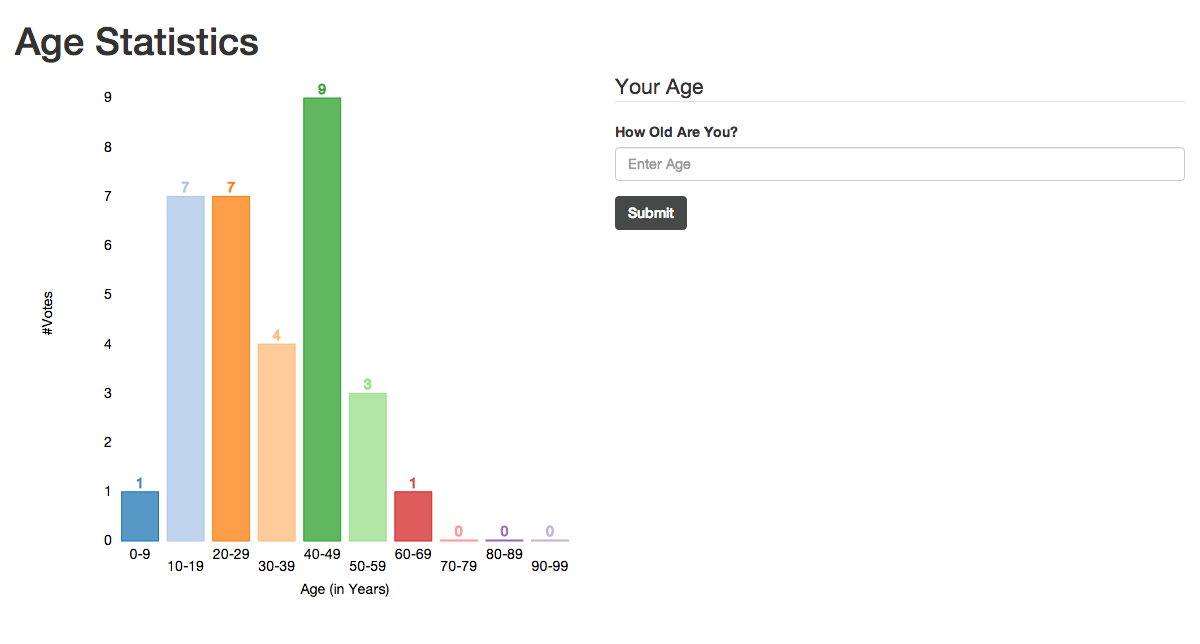
\includegraphics[width=\textwidth]{age_statistics.png}
\caption{Die Altersstatistiken-View mit Formular}
\label{fig:die_altersstatistiken_view_mit_formular}
\end{figure}

% subsubsection action_im_controller (end)

% subsection sammeln_der_statistiken (end)


% section beispielanwendung (end)


% chapter grundlagen (end)
%!TEX root = thesis.tex

\chapter{Reaktive Programmierung} % (fold)
\label{cha:reaktive_programmierung}

Reaktive Programmierung ist die Programmierung von reaktiven System.
Ein reaktives System ist ein System, das von seiner Umgebung kontinuierlich Daten empfängt und darauf reagiert.
In nebenläufigen Systemen können gleich mehrere solcher Datenströme unabhängig voneinander existieren \cite[vgl.][S.~1]{reactive_programming}.

Reaktive Prozesse haben die Eigenschaft, schrittweise, immer wenn sie neue Daten empfangen, ein Ergebnis aufzubauen.
Deshalb sind sie bei Berechnungen essentiell, bei denen nicht nur das Endergebnis wichtig ist, sondern auch die Schritte, die dazu geführt haben \cite[vgl.][S.~2]{reactive_programming1}.


\section{Futures und Promises} % (fold)
\label{sec:futures_und_promises}

Futures und Promises mit den Quellen \citealt{haller2013} und \citealt{typesafe2013}.

% section futures_und_promises (end)


\section{Streams} % (fold)
\label{sec:streams}

Streams sind inkrementelle Datenströme, die nicht-blockierendes Lesen erlauben und kombiniert und transformiert werden können.
Sie erlauben inkrementelle, deklarative und funktionale Datenverarbeitung mit voller Kontrolle über den Ressourcenverbrauch.
Anwendungsbeispiele für Streams sind beispielsweise die Implementierung von Web-Servern oder Datenkompression.
Die in diesem Kapitel vorgestellten Streams sind auch bekannt als Iteratee I/O.
Sie entstanden im Umfeld der Programmiersprache Haskell und wurden von Oleg Kiselyov vorgestellt \cite[vgl.][S.~19]{monad_reader}.
Als Quellen hierfür dienen \citealt{kiselyov2012}, \citealt{iteratee_io}, \citealt{monad_reader} und die Seiten der offiziellen Play-Dokumentation (\citealt{iteratees}, \cite{enumerators}, \cite{play_api_documentation}).


\subsection{Design} % (fold)
\label{sub:design}

Iteratee IO-Streams bestehen aus vier Komponenten.
\lstinline|Input|, \lstinline|Iteratee|, \lstinline|Enumerator| und \lstinline|Enumeratee|.
\lstinline|Input| beinhaltet die gestreamten Elemente.
\lstinline|Iteratee| konsumiert \lstinline|Input|-Elemente und dient somit als Datensenke.
\lstinline|Enumerator| generiert \lstinline|Input|-Elemente und dient somit als Datenquelle.
Und \lstinline|Enumeratee| transformiert einen \lstinline|Iteratee|.
Diese Komponenten und ihr jeweiliger Verwendungszweck wird in diesem Kapitel vorgestellt.


\subsubsection{Inputs} % (fold)
\label{ssub:design_inputs}

Die von der Datenquelle generierten Elemente werden in \lstinline|Input|s verpackt.
Der Datentyp \lstinline|Input| ist definiert, wie in Listing~\ref{lst:der_input_datentyp} gezeigt \cite[vgl.][Z.~224]{play_iteratee_source_code}.

\begin{lstlisting}[caption=Der Input-Datentyp, label=lst:der_input_datentyp]
sealed trait Input[+E]
object Input {
  case class El[+E](e: E) extends Input[E]
  case object Empty extends Input[Nothing]
  case object EOF extends Input[Nothing]
}
\end{lstlisting}

Der Datentyp ist über den kovarianten Typ \lstinline|E| der gehaltenen Elemente parametrisiert.
Kovarianz bedeutet, dass wenn \lstinline|F| ein spezialisierter Typ von \lstinline|E| ist, \lstinline|Input[F]| auch ein spezialisierter Typ von \lstinline|Input[E]| ist \cite[vgl.][S.~11]{variance}.
Dadurch wären beispielsweise sowohl \lstinline|Input[Cat]|, also auch \lstinline|Input[Dog]| Spezialisierungen von \lstinline|Input[Animal]|.
Wäre \lstinline|Input| nicht kovariant über den Typ der der gehaltenen Elemente, wären \lstinline|Input[Cat]|, \lstinline|Input[Dog]| und \lstinline|Input[Animal]| völlig unterschiedliche Typen.

Des Weiteren ist anzumerken, dass \lstinline|Input| ein \gls{adt} ist.
Ein \gls{adt} ist ein Datentyp mit mehreren, alternativen Konstruktoren, die jeweils eigene Felder besitzen.
Mittels Pattern Matching kann von einem Wert eines solchen Datentyps auf den verwendeten Konstruktor geschlossen werden \cite[vgl.][S.~14--15]{algebraic_data_type}.

In Scala werden algebraische Datentypen mit Hilfe von einem Marker-Trait und \lstinline|case|-Klassen und -Objekten implementiert.
Das Marker-Trait ist der algebraische Datentyp und die \lstinline|case|-Klassen und -Objekte sind die Konstruktoren.
Die Nutzung von \lstinline|case|-Klassen und -Objekten hat den Vorteil, dass diese mittels Pattern Matching zerlegt werden können.
Dadurch, dass das Marker-Trait \lstinline|sealed| ist, wird verhindert, dass von außerhalb der Quellcode-Datei weitere Konstruktoren hinzugefügt werden können \cite[vgl.][]{algebraic_data_type_scala}.
In diesem Fall besitzt der algebraische Datentyp \lstinline|Input| die Konstruktoren \lstinline|El|, \lstinline|Empty| und \lstinline|EOF|.
Der Konstruktor \lstinline|El| besitzt ein Feld, \lstinline|Empty| und \lstinline|EOF| besitzen keine Felder.

Für den Fall, dass die Datenquelle nicht erschöpft ist, existiert im Companion-Objekt die Unterklasse \lstinline|Input.El| mit dazugehöriger Konstruktormethode.
Diese Implementierung hält genau ein Element aus der Datenquelle.
Über die Entsprechung zu \lstinline|Input.Empty| in Kiselyovs Implementierung schreibt er "`[it] signifies a stream with no immediately available data but which is still continuing"' \cite[vgl.][]{iteratee_io}.
Außerdem findet es im Kontext von \lstinline|Iteratee|s Verwendung, um zu signalisieren, dass kein Teil der Eingabe übriggebliebenen ist.
Um zu signalisieren, dass die Datenquelle erschöpft ist, existiert das Objekt \lstinline|Input.EOF|.

Sowohl \lstinline|Input.Empty|, als auch \lstinline|Input.EOF| sind vom Typ \lstinline|Input[Nothing]|.
\lstinline|Nothing| ist ein besonderer Typ in Scala, der eine Spezialisierung jedes anderen Typs ist \cite[vgl.][S.~32]{scala_specification}.
Weil der Typparameter des \lstinline|Input|-Datentyps kovariant ist, lassen sich \lstinline|Input.Empty| und \lstinline|Input.EOF| mit jedem anderen \lstinline|Input| kombinieren.

Ein Wert vom Typ \lstinline|Input| hat also drei mögliche Zustände:
\begin{enumerate}
  \item Es gibt ein neues Element (\lstinline|Input.El|).
  \item Es gibt noch kein neues Element, doch die Datenquelle ist noch aktiv (\lstinline|Input.Empty|)
  \item Die Datenquelle ist erschöpft (\lstinline|Input.EOF|).
\end{enumerate}

% subsubsection design_inputs (end)


\subsubsection{Iteratees} % (fold)
\label{ssub:design_iteratees}

Die von der Datenquelle in \lstinline|Input|s verpackten Elemente werden von \lstinline|Iteratee|s konsumiert, um daraus ein Ergebnis aufzubauen.
\lstinline|Iteratee|s kapseln ihren Zustand \lstinline|Step|, der den Verarbeitungszustand widerspiegelt.
Der Typ des \lstinline|Step|-Zustands ist wie in Listing~\ref{lst:der_step_datentyp} gezeigt \cite[vgl.][Z.~256]{play_iteratee_source_code}.
\begin{lstlisting}[caption=Der Step-Datentyp, label=lst:der_step_datentyp]
sealed trait Step[E, +A]
object Step {
  case class Done[+A, E](a: A, remaining: Input[E])
    extends Step[E, A]
  case class Cont[E, +A](k: Input[E] => Iteratee[E, A])
    extends Step[E, A]
  case class Error[E](msg: String, input: Input[E])
    extends Step[E, Nothing]
}
\end{lstlisting}

Der algebraische Typ ist über die zwei Typen \lstinline|E| und \lstinline|A| parametrisiert.
\lstinline|E| ist der Typ der zu konsumierenden Elemente.
\lstinline|A| ist der Typ des zu berechnenden Ergebnisses.
\lstinline|A| ist kovariant, sodass auch Spezialisierungen von \lstinline|A| als Werte verwendet werden können.
Die Kovarianz über den Typ \lstinline|A| ermöglicht es auch hier wieder \lstinline|Nothing| in den Konstruktoren zu verwenden, wie im vorigen Kapitel beschrieben.

Ein \lstinline|Iteratee|, der mit seiner Berechnung fertig ist, ist im Zustand \lstinline|Step.Done|.
Ein solcher \lstinline|Iteratee| hält sein berechnetes Ergebnis und den Teil der letzten Eingabe, der nicht mehr verarbeitet wurde.
Ein \lstinline|Iteratee| in diesem Zustand nimmt keine weiteren Elemente an.
Häufig ist der Eingaberest \lstinline|Input.Empty|, weil die gesamte Eingabe konsumiert wurde.
Ein Beispiel für einen nicht leeren Eingaberest ist, wenn ein \lstinline|Iteratee| zeilenweise Dateiinhalte empfängt und darin nach einem Wort sucht.
Wenn das gesuchte Wort gefunden wurde, wird als Restwert der bisher nicht angesehene Rest der Zeile verwendet.

Ein \lstinline|Iteratee|, der noch kein Endergebnis berechnet hat, ist im Zustand \lstinline|Step.Cont|.
Das Argument von \lstinline|Step.Cont| ist die Schritt-Funktion \lstinline[breaklines=true]|Input[E] => Iteratee[E, A]|.
Die Eingabe der Schritt-Funktion ist ein \lstinline|Input| mit einem neuen zu verarbeitenden Element.
Die Ausgabe der Schritt-Funktion ist ein neuer \lstinline|Iteratee|, der den neuen Berechnungsstand nach dem Verarbeiten des Eingabeelements hält.
Diese Funktion wird als Continuation bezeichnet.
Eine Delimited Continuation repräsentiert den Rest einer Berechnung bis zu einem bestimmten Punkt \cite[vgl.][S.~1]{continuations}.
In diesem Fall berechnet die Continuation immer die Verarbeitung genau eines weiteren Elements.

Falls bei der Verarbeitung eines Elements ein Fehler auftritt, wird dies durch den Zustand \lstinline|Step.Error| signalisiert.
Ein solcher Fehler wird durch eine Fehlermeldung und durch das verursachende Eingabeelement dargestellt.
Beispielsweise kann ein \lstinline|Iteratee| nach dem Empfang eines \lstinline|Input.EOF|-Elements signalisieren, dass es noch mehr Daten benötigt.
%In diesem Fall kann das System versuchen doch noch mehr Daten zu finden, sodass der \lstinline|Iteratee| erfolgreich zu einem Ergebnis kommen kann.

Ein \lstinline|Iteratee| hat also einen Verarbeitungszustand vom Typ \lstinline|Step| mit drei möglichen Zuständen:
\begin{enumerate}
  \item Es wurde erfolgreich ein Ergebnis berechnet (\lstinline|Step.Done|).
  \item Es werden weitere Daten zur Berechnung benötigt (\lstinline|Step.Cont|).
  \item Es ist ein Fehler aufgetreten (\lstinline|Step.Error|).
\end{enumerate}

Außerdem ist anzumerken, dass der \lstinline|Iteratee|-Typ ist eine Monade.
Dadurch ist es möglich, einen beliebigen Wert in die Monade zu heben, die dann im \lstinline|Step.Done|-Zustand ist.
Auch kann ein erfolgreich berechneter Wert innerhalb der Monade transformiert werden.

% subsubsection design_iteratees (end)


\subsubsection{Enumerators} % (fold)
\label{ssub:design_enumerators}

Ein \lstinline|Enumerator| ist die Datenquelle, die ihre Daten, in \lstinline|Input|s verpackt, bereitstellt.
Der Datentyp \lstinline|Enumerator| ist definiert, wie in Listing~\ref{lst:der_enumerator_datentyp} vereinfacht dargestellt \cite[vgl.][]{play_enumerator_source_code}.
\begin{lstlisting}[caption=Der Enumerator-Datentyp, label=lst:der_enumerator_datentyp]
trait Enumerator[E] {
  def apply[A](i: Iteratee[E, A]): Future[Iteratee[E, A]]
}
\end{lstlisting}

Ein \lstinline|Enumerator| ist eine Funktion von \lstinline|Iteratee| nach \lstinline|Iteratee| und ist über die Typen des übergebenen \lstinline|Iteratee|s parametrisiert.
Der Eingabewert ist der \lstinline|Iteratee|, an den die generierten Elemente gesendet werden.
Der Rückgabewert ist der übergebene \lstinline|Iteratee| nach Fertigstellung oder Abbruch seiner Berechnung.
Der zurückgegebene \lstinline|Iteratee| befindet sich in der \lstinline|Future|-Monade.

Bei der Anwendung dieser Funktion werden dem \lstinline|Iteratee| so lange Daten übergeben, bis die Datenquelle erschöpft ist, oder bis der \lstinline|Iteratee| keine Daten mehr annimmt.
Die Herkunft der Daten, die der \lstinline|Enumerator| an den \lstinline|Iteratee| sendet, ist beliebig.
Weil der Rückgabetyp sich in der \lstinline|Future|-Monade befindet können auch zeitintensive Berechnungen durchgeführt werden, ohne den Programmfluss zu unterbrechen.
Dadurch ist es beispielsweise möglich, die Daten aus Dateien oder dem Netzwerk zu empfangen.

% subsubsection design_enumerators (end)


\subsubsection{Enumeratees} % (fold)
\label{ssub:design_enumeratees}

Ein \lstinline|Enumeratee| ist ein Stream-Transformator, der \lstinline|Iteratee|s eines bestimmten Element-Typs zu \lstinline|Iteratee|s eines anderen Element-Typs konvertiert.
Der Datentyp \lstinline|Enumeratee| ist definiert, wie in Listing~\ref{lst:der_enumeratee_datentyp} vereinfacht dargestellt \cite[vgl.][]{play_enumeratee_source_code}.
\begin{lstlisting}[caption=Der Enumeratee-Datentyp, label=lst:der_enumeratee_datentyp]
trait Enumeratee[From, To] {
  def apply[A](inner: Iteratee[To, A]):
    Iteratee[From, Iteratee[To, A]]
}
\end{lstlisting}

Ein \lstinline|Enumeratee| ist eine Funktion von \lstinline|Iteratee| nach \lstinline|Iteratee|.
Der Eingabewert ist der zu transformierende \lstinline|Iteratee| vom inneren Element-Typ \lstinline|To|.
Der Ausgabewert ist ein \lstinline|Iteratee| vom äußeren Element-Typ \lstinline|From|.
Der neue \lstinline|Iteratee| nimmt Elemente vom Typ \lstinline|From| an und transformiert sie nach \lstinline|To|.
Diese transformierten Werte werden dann an den ursprünglichen \lstinline|Iteratee| weitergegeben.

Elemente vom Typ \lstinline|From| heißen äußere Elemente, weil sie vom resultierenden \lstinline|Iteratee| zuerst empfangen werden.
Elemente vom Typ \lstinline|To| heißen innere Elemente, weil sie zum \lstinline|Iteratee| gehören, das sich im Rückgabetyp des resultierenden \lstinline|Iteratee|s befindet.
Die Elemente des äußeren \lstinline|Iteratees| werden nach der Transformation an den inneren \lstinline|Iteratee| weitergereicht.

Die Transformation muss dabei aber nicht ein Element nach genau einem anderen Element abbilden.
Ein äußeres Element \lstinline|From| kann zu einem, keinem oder auch mehreren inneren Elementen \lstinline|To| abgebildet werden.
Genauso ist es möglich, dass mehrere äußere Elemente zu einem inneren Element zusammengefasst werden.

Ein \lstinline|Enumeratee| kann auch als \lstinline|Enumerator| betrachtet werden.
Dies kommt daher, dass \lstinline|Iteratee|s Monaden sind.
Ein \lstinline|Enumeratee| ist ein \lstinline|Enumerator|, dessen Ergebnis nicht in der \lstinline|Future|-Monade, sondern in der \lstinline|Iteratee|-Monade liegt.
Jeder \lstinline|Enumeratee| ist auch ein \lstinline|Iteratee|, wenn man seinen Rückgabewert betrachtet, der vom Typ \lstinline|Iteratee| ist.
Ein \lstinline|Enumeratee| ist also sowohl in der Rolle eines \lstinline|Iteratee|s, als auch in der Rolle eines \lstinline|Enumerator|s.
Er ist ein \lstinline|Iteratee| des äußeren Typs \lstinline|From| und ein \lstinline|Enumerator| des inneren Typs \lstinline|To|, weil er Elemente des äußeren Typs konsumiert und Elemente des inneren Typs generiert.

% subsubsection design_enumeratees (end)


\subsubsection{Komposition} % (fold)
\label{ssub:komposition}

Bei der Komposition werden zwei oder mehr \lstinline|Iteratee|s oder \lstinline|Enumerator|s zu einem neuen \lstinline|Iteratee| oder \lstinline|Enumerator| kombiniert.
Es gibt hierbei zwei prinzipielle Arten der Komposition.
Diese Arten sind die sequentielle und die parallele Komposition.

\paragraph{Komposition von Iteratees} % (fold)
\label{par:komposition_von_iteratees}\mbox{} % force new line

Sequenzielle Komposition zweier \lstinline|Iteratee|s funktioniert noch folgendem Prinzip:
Zuerst wird der erste \lstinline|Iteratee| angewendet, bis er keine Elemente mehr annimmt oder die Datenquelle erschöpft ist.
Dann wird der zweite \lstinline|Iteratee| auf die noch übrigen Elemente der Datenquelle angewendet, bis auch dieser \lstinline|Iteratee| keine Elemente mehr annimmt, oder die Datenquelle erschöpft ist.
Anschließend werden die Ergebnisse beider \lstinline|Iteratee|s kombiniert, z.~B. als Paar. % Iteratee#map/flatMap

Bei der parallelen Komposition werden die Elemente der Datenquelle an beide \lstinline|Iteratee|s weitergegeben.
Dies geschieht im Gegensatz zur sequentiellen Komposition allerdings ohne, dass zuerst ein \lstinline|Iteratee| vollständig beendet sein muss.
Es ist möglich \lstinline|Iteratee|s so zu kombinieren, dass der resultierende \lstinline|Iteratee| eine Datenquelle auf mehrere Datensenken abbildet.
Die Datensenken sind hierbei die kombinierten \lstinline|Iteratee|s.
Beispielsweise können die Elemente der Datenquelle immer an beide \lstinline|Iteratee|s weitergegeben werden, um die Ergebnisse beider \lstinline|Iteratee|s anschließend als Paar zu zusammenzufassen. % Enumeratee.zip/zipWith

% paragraph komposition_von_iteratees (end)

\paragraph{Komposition von Enumerators} % (fold)
\label{par:komposition_von_enumerators}\mbox{} % force new line

Die sequentielle Komposition zweier \lstinline|Enumerator|s erfolgt ähnlich, wie die sequentielle Kompositionen von \lstinline|Iteratee|s.
Der resultierende \lstinline|Enumerator| generiert erst alle Elemente des ersten \lstinline|Enumerator|s und dann alle Elemente des zweiten \lstinline|Enumerator|s.
Die sequentielle Komposition von \lstinline|Enumerator|s entspricht also der Verkettung ihrer Ausgaben. %Enumerator.andThen

Parallele Komposition von \lstinline|Enumerator|s bedeutet, dass nicht erst ein \lstinline|Enumerator| erschöpft sein muss, bevor Daten generiert werden, die dem anderen \lstinline|Enumerator| entstammen.
Dabei muss nicht erst ein \lstinline|Enumerator| erschöpft sein, bevor Daten generiert werden, die aus einem anderen \lstinline|Enumerator| entstammen.
Eine Möglichkeit ist, dass die Reihenfolge der Elemente dadurch bestimmt wird, welcher \lstinline|Enumerator| zuerst ein neues Element zur Verfügung stellt. % Enumerator.interleave

% paragraph komposition_von_enumerators (end)

% subsubsection komposition (end)


% subsection design (end)


\subsection{Anwendung} % (fold)
\label{sub:anwendung}

Im vorigen Kapitel zum Design der \lstinline|Iteratee|-Streams wurden die Grundkomponenten des Moduls vorgestellt.
In diesem Kapitel soll ihr Einsatz mit Hilfe von konkreten Code-Beispielen gezeigt werden.
Es wird werden häufig mehrere Möglichkeiten für die Verwendung der einzelnen Komponenten erläutert, um die unterschiedlichen Abstraktionsschichten zu verdeutlichen.
Die Codebeispiele stammen, sofern nicht anders vermerkt, vom Autoren.


\subsubsection{Iteratees} % (fold)
\label{sssec:iteratees}

Plays \lstinline|Iteratee|s bilden einen Container um ihren \lstinline|Step|-Zustand.
Dadurch werden, wie bei objektorientierten Sprachen üblich\todo{Zitat}, Daten und Operationen gebündelt.
Die elementare Methode dieses Traits ist \lstinline|fold|.
Die Signatur dazu ist in Listing~\ref{lst:fold_signatur} zu lesen.
\begin{lstlisting}[caption=Die Signatur von fold, label=lst:fold_signatur]
def fold[B](folder: Step[E, A] => Future[B]): Future[B]
\end{lstlisting}

Mit Hilfe von \lstinline|fold| lässt sich der Zustand des \lstinline|Iteratee|s transformieren.
Deshalb sind sehr viele Methoden des \lstinline|Iteratee|-Traits auf Basis von \lstinline|fold| definiert.
Durch Übergabe eines \lstinline|Step|-Werts an die \lstinline|folder|-Funktion bestimmt die konkrete \lstinline|Iteratee|-Implementierung, wie mit übergebenen Elementen umzugehen ist und ob überhaupt weitere Elemente akzeptiert werden.
Nur durch die im \lstinline|Step|-Wert befindliche Eingabeverarbeitung kann ein \lstinline|Iteratee| neue Elemente empfangen.
Dadurch wird nach und nach der zu berechnende Wert aufgebaut.

\paragraph{Iteratees erstellen} % (fold)
\label{par:iteratees_erstellen}\mbox{} % force new line

Es gibt drei Möglichkeiten, einen neuen \lstinline|Iteratee| zu erstellen.
\begin{enumerate}
  \item Durch Erstellung einer neuen Klasse, die das \lstinline|Iteratee|-Trait implementiert.
  \item Durch Benutzung einer Konstruktormethode analog zu den \lstinline|Step|-Zuständen (\lstinline|Done|, \lstinline|Cont| und \lstinline|Error|).
  \item Durch Benutzung einer Konstruktormethode des Companion-Objekts (\lstinline|fold|, \lstinline|foreach|, u.~a.).
\end{enumerate}

Zu Demonstrationszwecken soll im Folgenden ein \lstinline|Iteratee| erstellt werden, der alle empfangenen Elemente aufsummiert.
Es wird dabei nach jeder der drei möglichen Varianten implementiert.

\subparagraph{Erstellung durch Vererbung} % (fold)
\label{subp:erstellung_durch_vererbung}\mbox{} % force new line

Die erste Variante ist, von \lstinline|Iteratee| zu erben und die \lstinline|fold|-Methode zu implementieren.
Dies erfordert viel Schreibarbeit, weil nur die sehr generische \lstinline|fold|-Methode verwendet werden kann.
Der Code dazu ist in Listing~\ref{lst:iteratee_durch_vererbung} zu sehen.

\begin{lstlisting}[caption=Erstellung eines Iteratees durch Vererbung, label=lst:iteratee_durch_vererbung]
case class SumIteratee(sum: Int = 0) extends Iteratee[Int, Int] {
  def fold[B](folder: Step[Int, Int] => Future[B]): Future[B] = {
    folder(Step.Cont {
      case Input.El(i) => SumIteratee(sum + i)
      case Input.Empty => this
      case Input.EOF   => new Iteratee[Int, Int] {
        def fold[B](folder: Step[Int, Int] => Future[B]) = {
          folder(Step.Done(sum, Input.EOF))
        }
      }
    })
  }
}

val sumIterateeFromInheritance: Iteratee[Int, Int] = SumIteratee()
\end{lstlisting}

Der \lstinline|folder|-Funktion muss der aktuelle \lstinline|Step|-Zustand übergeben werden.
Diese Funktion soll den \lstinline|Iteratee| dann mit Elementen versorgen.
Anschließend soll der \lstinline|folder| dann aus dem finalen Zustand ein Ergebnis berechnen.
Solange noch weitere Elemente kommen können, also solange kein \lstinline|Input.EOF|-Element empfangen wurde, geht der \lstinline|Iteratee| in einen neuen \lstinline|Cont|-Zustand über.
Bei diesem Zustandsübergang wird auch die interne Berechnung fortgesetzt.
Es wird also in einen \lstinline|Cont|-Zustand übergegangen, der die aktualisierte Summe hält.
Wenn ein leeres Element (\lstinline|Input.Empty|) verarbeitet werden soll, wird der \lstinline|Iteratee| unverändert zurückgegeben, weil sich an der Gesamtsumme nichts geändert hat.
Sobald keine weiteren Elemente mehr kommen können, wird die Berechnung beendet und ein \lstinline|Iteratee| an den \lstinline|folder| übergeben, der sich immer im \lstinline|Done|-Zustand befindet.

% subparagraph erstellung_durch_vererbung (end)

\subparagraph{Erstellung durch Konstruktormethode} % (fold)
\label{subp:erstellung_durch_konstruktormethode}\mbox{} % force new line

Die zweite Möglichkeit, einen \lstinline|Iteratee| zu erstellen, ist mit Hilfe einer der Konstruktormethoden.
Es gibt die Konstruktormethoden \lstinline|Done|, \lstinline|Cont| und \lstinline|Error|, die jeweils einen \lstinline|Iteratee| im gleichnamigen \lstinline|Step|-Zustand erstellen.
Jede diese Methoden nimmt auch die gleichen Argumente, wie ihr Pendant.
Der Code, der einen \lstinline|Iteratee| mit Hilfe dieser Methoden erstellt, ist in Listing~\ref{lst:iteratee_durch_konstruktormethode} zu sehen.

\begin{lstlisting}[caption=Erstellung eines Iteratees durch eine Konstruktormethode, label=lst:iteratee_durch_konstruktormethode]
def sumIteratee(sum: Int = 0): Iteratee[Int, Int] = Cont {
  case Input.El(i) => sumIteratee(sum + i)
  case Input.Empty => sumIteratee(sum)
  case Input.EOF   => Done(sum, Input.EOF)
}

val sumIterateeFromConstructor: Iteratee[Int, Int] = sumIteratee()
\end{lstlisting}

Der Code ist dem in \nameref{lst:iteratee_durch_vererbung} vorgestellten Code sehr ähnlich.
Im Gegensatz dazu muss hier jedoch nicht mehr explizit von \lstinline|Iteratee| geerbt und die \lstinline|fold|-Methode implementiert werden.
Dies macht den Code schon wesentlich kürzer und einfacher.
Der Code ist auf die elementaren Aufgaben reduziert und es ist nun klar zu erkennen, was bei welcher Eingabe geschieht.

% subparagraph erstellung_durch_konstruktormethode (end)

\subparagraph{Erstellung durch Konstruktormethode im Companion-Objekt} % (fold)
\label{subp:erstellung_durch_konstruktormethode_im_companion_objekt}\mbox{} % force new line

Die dritte und letzte Möglichkeit nutzt eine problemspezifische Konstruktormethode im Companion-Objekt.
Das Aufsummieren einer Menge von Zahlen lässt sich sehr einfach mit Hilfe eines Folds implementieren\todo{Erklären, was ein Fold ist}.
Das \lstinline|Iteratee|-Companion-Objekt beinhaltet u.~a. die \lstinline|fold|-Konstruktormethode, die für solche Operationen gedacht ist.
Durch Einsatz dieser Methode wird die Lösung, wie in Listing~\ref{lst:iteratee_durch_hilfsmethode} zu erkennen, zum Einzeiler.
Vom Filtern der unterschiedlichen \lstinline|Input|-Typen ist hierbei abstrahiert und es muss sich nur noch um tatsächliche Eingabeelemente gekümmert werden.

\begin{lstlisting}[caption=Erstellung eines Iteratees durch Konstruktormethode im Companion-Objekt, label=lst:iteratee_durch_hilfsmethode]
val sumIterateeFromHelper: Iteratee[Int, Int] =
  Iteratee.fold(0)(_ + _)
\end{lstlisting}

Eine weitere hilfreiche Konstruktormethode ist \lstinline|getChunks|.
Diese Methode gibt einen \lstinline|Iteratee| zurück, der alle empfangenen Elemente in einer Liste sammelt.
Der Typ dieses \lstinline|Iteratee|s ist entsprechend \lstinline|Iteratee[E, List[E]]|.
Dieser \lstinline|Iteratee| wird im Folgenden zu Veranschaulichungszwecken an einigen Stellen dieser Arbeit verwendet.

% subparagraph erstellung_durch_konstruktormethode_im_companion_objekt (end)

% paragraph iteratees_erstellen (end)

\paragraph{Iteratees ausführen} % (fold)
\label{par:iteratees_ausfuehren}\mbox{} % force new line

Um die \lstinline|Iteratee|s mit Daten zu versorgen, existiert, wie in \nameref{par:iteratees_erstellen} beschrieben, die Methode \lstinline|fold|.
\lstinline|fold| nimmt als Argument eine Funktion \lstinline|folder| vom Typ \lstinline[breaklines=true]|Step[E, A] => Future[B]|.
Diese Funktion übergibt ein Element an den \lstinline|Iteratee| und muss daraufhin den Zustand des neuen \lstinline|Iteratee|s überprüfen, ob weitere Elemente akzeptiert werden.
Erst nach dieser Analyse kann entschieden werden, ob ein weiteres Element übergeben wird oder nicht.
In Listing~\ref{lst:iterateeausfuehrung_durch_folder} wird gezeigt, wie dies implementiert werden kann.

\begin{lstlisting}[caption=Ausführung eines Iteratees durch folder-Funktion, label=lst:iterateeausfuehrung_durch_folder]
def folder(xs: Int*)(step: Step[Int, Int]): Future[Int] = {
  def folder_(xs: List[Int])(step: Step[Int, Int]): Future[Int] =
    xs match {
      case Nil => step match {
        case Step.Cont(k) => k(Input.EOF).fold {
          case Step.Done(sum, Input.EOF) => Future(sum)
          case _ => Future.failed(new Exception("invalid state"))
        }
        case _ => Future.failed(new Exception("invalid state"))
      }
      case x :: xs => step match {
        case Step.Cont(k) => k(Input.El(x)).fold(folder_(xs))
        case _ => Future.failed(new Exception("invalid state"))
      }
    }

  folder_(xs.toList)(step)
}

val sumResult: Future[Int] =
  sumIterateeFromHelper.fold(folder(1, 4, -2))
// sumResult = Future.successful(3)
\end{lstlisting}

Das Übergeben von Daten mittels der \lstinline|fold|-Methode ist, wie in Listing~\ref{lst:iterateeausfuehrung_durch_folder} zu erkennen, recht aufwändig.
Dies kommt daher, dass zwei Zustände geprüft werden müssen.
Zum Einen muss der Zustand der Eingabemenge geprüft werden, ob noch Elemente existieren, die an den \lstinline|Iteratee| übergeben werden sollen.
Zum Anderen muss sichergestellt werden, dass der \lstinline|Iteratee| sich korrekt verhält.
D.~h. solange kein \lstinline|Input.EOF| gesendet wurde, muss der \lstinline|Iteratee| weitere Elemente annehmen und sobald ein \lstinline|Input.EOF| gesendet wurde, darf der \lstinline|Iteratee| keine Elemente mehr annehmen.
Nur wenn all diese Voraussetzungen erfüllt wurden, kann am Ende das Ergebnis dem \lstinline|Iteratee| im \lstinline|Step.Done|-Zustand entnommen werden.
Durch Verwendung von \lstinline|Enumerator|s wird dies allerdings wesentlich einfacher.

% paragraph iteratees_ausfuehren (end)

% subsubsection iteratees (end)

\subsubsection{Enumerators} % (fold)
\label{ssub:enumerators}

Mit Hilfe von \lstinline|Enumerator|s können auf einfache Weise Daten an \lstinline|Iteratee|s übergeben werden.
In diesem Kapitel werden Anwendung und Funktionsweise von \lstinline|Enumerator|s gezeigt.
Es wird erklärt, auf welche Arten \lstinline|Enumerator|s erstellt werden können, und wie sie genutzt werden können, um Daten an \lstinline|Iteratee|s zu übergeben.

\paragraph{Enumerators erstellen} % (fold)
\label{par:enumerators_erstellen}\mbox{} % force new line

Es gibt drei unterschiedliche Techniken, einen \lstinline|Enumerator| zu erstellen.
\begin{enumerate}
  \item Durch Erstellung einer neuen Klasse, die das \lstinline|Enumerator|-Trait implementiert.
  \item Durch Benutzung einer Konstruktormethode im Companion-Objekt im Companion-Objekt (\lstinline|apply|, \lstinline|generateM|, u.~a.).
  \item Durch Benutzung einer Konstruktormethode im \lstinline|Concurrent|-Objekt (\lstinline|broadcast|, \lstinline|unicast|, u.~a.).
\end{enumerate}

Im Folgenden werden alle Herangehensweisen vorgestellt, um Zahlen für den im vorigen Kapitel vorgestellten Summierungs-\lstinline|Iteratee| zu generieren.

\subparagraph{Erstellung durch Vererbung} % (fold)
\label{subp:enumeratorerstellung_durch_vererbung}\mbox{} % force new line

Bei der Erstellung eines \lstinline|Enumerator|s durch Vererbung, muss das \lstinline|Enumerator|-Trait implementiert werden.
Alles, was dafür nötig ist, ist die \lstinline|apply|-Methode zu implementieren.
Innerhalb dieser Methode wird der übergebene \lstinline|Iteratee| mit Hilfe seiner \lstinline|fold|-Methode befüllt, wie in Listing~\ref{lst:enumeratorerstellung_durch_vererbung} zu sehen.

\begin{lstlisting}[caption=Erstellung eines Enumerators durch Vererbung, label=lst:enumeratorerstellung_durch_vererbung]
case class NumberEnumerator(xs: Int*) extends Enumerator[Int] {
  def apply[A](iteratee: Iteratee[Int, A]):
      Future[Iteratee[Int, A]] = {
    xs.foldLeft(Future(iteratee)) { (futureIteratee, x) =>
      futureIteratee.flatMap { iteratee =>
        iteratee.fold {
          case Step.Cont(k) => Future(k(Input.El(x)))
          case _ => Future(iteratee)
        }
      }
    }
  }
}

val numberEnumeratorFromInheritance: Enumerator[Int] =
  NumberEnumerator(1, 4, -2)
\end{lstlisting}

Alles was ein \lstinline|Enumerator| zu tun hat, ist seine Daten an den übergebenen \lstinline|Iteratee| zu übergeben.
Dieses Vorgehen ist in diesem Beispiel als Fold über den \lstinline|Iteratee| implementiert.
Es wird immer ein Element an den \lstinline|Iteratee| übergeben und der resultierende \lstinline|Iteratee| als neues Zwischenergebnis verwendet.
Falls der \lstinline|Iteratee| keine weiteren Elemente akzeptiert, obwohl noch Elemente übrig sind, wird dieser als Endergebnis verwendet.
Das hier vorgestellte Verfahren ist in leicht abgewandelter Form der Implementierung von \lstinline|Enumerator.apply| entnommen \cite[vgl.][Z.~663 und Z.~690]{play_enumerator_source_code}.

% subparagraph enumeratorerstellung_durch_vererbung (end)

\subparagraph{Erstellung durch Konstruktormethode im Companion-Objekt} % (fold)
\label{subp:erstellung_durch_konstruktormethode_im_companion-object}\mbox{} % force new line

Die zweite Variante, einen \lstinline|Enumerator| zu erstellen, ist mit Hilfe einer der Konstruktormethoden des Companion-Objekts.
Hierfür gibt es mehrere hilfreiche Methoden, die an dieser Stelle aber nicht alle vorgestellt werden können.
Stattdessen wird exemplarisch eine Methode vorgestellt, die auch in den folgenden Beispielen verwendet werden wird.

Die hier vorgestellte Methode ist die \lstinline|apply|-Methode des Companion-Objekts mit der Signatur \lstinline[breaklines=true]|def apply[E](in: E*): Enumerator[E]|.
Diese Methode nimmt als Parameter beliebig viele Elemente eines Typs und wird diese bei Anwendung in \lstinline|Input|-Elemente verpacken und an den \lstinline|Iteratee| übergeben.
Wie der \lstinline|Enumerator| mit dieser Methode erstellt wird, ist in Listing~\ref{lst:enumeratorerstellung_durch_apply} zu sehen.

\begin{lstlisting}[caption=Erstellung eines Enumerators durch die apply-Konstruktormethode, label=lst:enumeratorerstellung_durch_apply]
val numberEnumeratorFromApply: Enumerator[Int] =
  Enumerator(1, 4, -2)
\end{lstlisting}

% subparagraph erstellung_durch_konstruktormethode_im_companion-object (end)

\subparagraph{Erstellung durch Konstruktormethode im Concurrent-Objekt} % (fold)
\label{subp:erstellung_durch_konstruktormethode_im_concurrent_objekt}\mbox{} % force new line

Das Objekt \lstinline|Concurrent| stellt weitere Konstruktoren für \lstinline|Enumerator|s bereit.
Unter anderem beinhaltet dieses Objekt die Methode \lstinline|unicast|, die imperatives schreiben auf einen \lstinline|Iteratee| erlaubt.
Die Signatur von \lstinline|unicast| ist wie in Listing~\ref{lst:unicast_signatur} dargestellt.

\begin{lstlisting}[caption=Die Signatur von Concurrent.unicast, label=lst:unicast_signatur]
def unicast[E](
  onStart: (Channel[E]) => Unit,
  onComplete: => Unit,
  onError: (String, Input[E]) => Unit): Enumerator[E]
\end{lstlisting}

Die Methode nimmt als Argumente drei Funktionen: \lstinline|onStart|, \lstinline|onComplete| und \lstinline|onError|.
\lstinline|onStart| wird immer aufgerufen, wenn die \lstinline|apply|-Methode des \lstinline|Enumerator|s aufgerufen wird.
\lstinline|onComplete| wird aufgerufen, wenn der \lstinline|Iteratee| in den \lstinline|Step.Done|-Zustand übergegangen ist.
\lstinline|onError| wird aufgerufen, wenn der \lstinline|Iteratee| in den \lstinline|Step.Error|-Zustand übergegangen ist.
Die letzten beiden Funktionen sind optionale Argumente.

Die \lstinline|onStart|-Funktion nimmt ein Argument vom Typ \lstinline|Channel|.
Ein \lstinline|Channel| hat u.~a. die Methoden \lstinline[breaklines=true]|def push(item: E): Unit| und \lstinline[breaklines=true]|def end(): Unit|.
Diese Methoden erlauben es, ein Element an das verbundene \lstinline|Iteratee| zu übergeben, bzw. zu signalisieren, dass der \lstinline|Enumerator| keine weiteren Elemente mehr hat.

Um mit Hilfe der \lstinline|unicast|-Methode einen Zahlen generierenden \lstinline|Enumerator| zu erstellen, wird nur die \lstinline|onStart|-Funktion benötigt.
Diese Funktion ist dafür zuständig, die Elemente an den \lstinline|Channel| und somit an den verbundenen \lstinline|Iteratee| zu übergeben.
Wichtig ist dabei jedoch, dass nach Übergabe aller Zahlen der \lstinline|Channel| wieder geschlossen wird.
Andernfalls wird niemals signalisiert, dass keine weiteren Elemente mehr kommen und der \lstinline|Iteratee| wird nicht in den \lstinline|Step.Done|-Zustand übergehen.
Die Implementation dazu ist in Listing~\ref{lst:enumeratorerstellung_durch_unicast} zu sehen.

\begin{lstlisting}[caption=Erstellung eines Enumerators durch die unicast-Konstruktormethode, label=lst:enumeratorerstellung_durch_unicast]
def numberEnumerator(xs: Int*): Enumerator[Int] = {
  Concurrent.unicast { channel =>
    xs.foreach(channel.push(_))
    channel.end
  }
}

val numberEnumeratorFromUnicast: Enumerator[Int] =
      numberEnumerator(1, 4, -2)
\end{lstlisting}

% subparagraph erstellung_durch_konstruktormethode_im_concurrent_objekt (end)

% paragraph enumerators_erstellen (end)

\paragraph{Anwendung auf Iteratees} % (fold)
\label{par:anwendung_auf_iteratees}\mbox{} % force new line

\lstinline|Enumerator|s sind, wie in Kap.~\ref{ssub:design_enumerators} erklärt, Funktionen.
Das Ergebnis der Anwendung einer solchen \lstinline|Enumerator|-Funktion ist der übergebene \lstinline|Iteratee| nach Konsum der Elemente in der \lstinline|Future|-Monade.
Ein Beispiel für diese ersten Schritte ist in Listing~\ref{lst:enumeratoranwendung1} zu sehen.

\begin{lstlisting}[caption=Anwendung eines Enumerators auf einen Iteratee, label=lst:enumeratoranwendung1]
val iteratee: Iteratee[Int, Int] = Iteratee.fold(0)(_ + _)
val enumerator: Enumerator[Int] = Enumerator(1, 4, -2)
val futureIterateeAfterApplication: Future[Iteratee[Int, Int]] =
  enumerator(iteratee)
\end{lstlisting}


Um mit dem neuen \lstinline|Iteratee| weiterzuarbeiten wäre es möglich, alle weiteren Operationen innerhalb der \lstinline|Future|-Monade durchzuführen.
Weil es aber eine Indirektion bedeuten würde, \lstinline|Iteratee|s innerhalb von \lstinline|Future|s zu bearbeiten, ist es möglich einen Wert vom Typ \lstinline|Future[Iteratee[E, A]]| in einen Wert vom Typ \lstinline|Iteratee[E, A]| zu transformieren.
Beide Typen haben die gleiche Bedeutung, indem sie für ein Ergebnis stehen, das möglicherweise noch nicht vorhanden ist.
Weil ein \lstinline|Iteratee| innerhalb der \lstinline|Future|-Monade aus diesem Betrachtungswinkel aber redundant ist, existiert die Methode \lstinline|Iteratee.flatten|.


Nachdem ein \lstinline|Enumerator| alle Elemente an einen \lstinline|Iteratee| übergeben hat, sendet er allerdings kein \lstinline|Input.EOF|-Element.
Dadurch ist es möglich, mehrere \lstinline|Enumerator|s auf einen \lstinline|Iteratee| anzuwenden, worauf in Kap.~\ref{subp:anwendung_sequentielle_komposition_von_enumerators} näher eingegangen wird.
Um ein \lstinline|Input.EOF|-Element an ein \lstinline|Iteratee| zu senden und anschließend das berechnete Ergebnis zu erhalten, wird die \lstinline|run|-Methode aus dem \lstinline|Iteratee|-Trait aufgerufen.
Eine Weiterführung des zuvor begonnenen \lstinline|Enumerator|-Beispiels ist in Listing~\ref{lst:enumeratoranwendung2} zu finden.
In diesem Beispiel werden die beiden oben beschriebenen Techniken angewendet, um die berechnete Summe aus dem \lstinline|Iteratee| zu extrahieren.

\begin{lstlisting}[caption=Extrahierung des Ergebnisses aus einem Iteratee, label=lst:enumeratoranwendung2]
val iterateeAfterApplication: Iteratee[Int, Int] =
  Iteratee.flatten(futureIterateeAfterApplication)

val futureResult: Future[Int] = iterateeAfterApplication.run
\end{lstlisting}

Mit Hilfe der Methode \lstinline|Enumerator.run| ist es außerdem möglich, \lstinline|Enumerator|anwendung und Ergebnisextraktion zusammenzufassen.
Diese Methode hat die Signatur \lstinline[breaklines=true]|def run[A](i: Iteratee[E, A]): Future[A]|.
Unter Einsatz dieser Methode wird die Verarbeitung im Aufsummierungsbeispiel, wie in Listing~\ref{lst:enumeratoranwendung3} zu sehen, auf einen Befehl verkürzt.

\begin{lstlisting}[caption=Anwendung eines Enumerators mit gleichzeitiger Ergebnisextrahierung, label=lst:enumeratoranwendung3]
val futureResult2: Future[Int] = enumerator.run(iteratee)
\end{lstlisting}

% paragraph anwendung_auf_iteratees (end)

% subsubsection enumerators (end)


\subsubsection{Enumeratees} % (fold)
\label{ssub:enumeratees}

\lstinline|Enumeratee|s sind Stream-Transformatoren, die \lstinline|Iteratee|s eines Typs zu \lstinline|Iteratee|s eines anderen Typs transformieren.
Sie sind, wie in Kap.~\ref{ssub:design_enumeratees} erklärt, Funktionen von \lstinline|Iteratee| nach \lstinline|Iteratee|.
Das Ergebnis des resultierenden \lstinline|Iteratee|s ist wiederum ein \lstinline|Iteratee|.
Und zwar ist es der ursprünglichen \lstinline|Iteratee| nach Empfang der Elemente.
Plays \lstinline|Enumeratee|s ermöglichen es allerdings auch \lstinline|Enumerator|s und andere \lstinline|Enumeratee|s zu transformieren.
In diesem Kapitel wird beschrieben, wie eigene \lstinline|Enumeratee|s erstellt und wie sie auf \lstinline|Iteratee|s, \lstinline|Enumerator|s und \lstinline|Enumeratee|s angewendet werden können.

\paragraph{Erstellung von Enumeratees} % (fold)
\label{par:erstellung_von_enumeratees}\mbox{} % force new line

Es gibt drei Möglichkeiten, einen \lstinline|Enumeratee| zu erstellen.

\begin{enumerate}
  \item Durch Erstellung einer neuen Klasse, die das \lstinline|Enumeratee|-Trait implementiert.
  \item Durch Benutzung einer Konstruktormethode des Companion-Objekts (\lstinline|map|, \lstinline|filter|, u.~a.)
  \item Durch Benutzung einer Konstruktormethode des \lstinline|Traversable|-Objekts (\lstinline|take|, \lstinline|drop|, u.~a.)
\end{enumerate}

Im Folgenden werden die ersten beiden Möglichkeiten vorgestellt und mit Beispielen veranschaulicht.
In den Beispielen wird ein \lstinline|Enumeratee| implementiert, der die Zahlen eines \lstinline|Iteratee[Int, Int]| mit 2 multipliziert.
Die dritte Möglichkeit ist an dieser Stelle nur der Vollständigkeit halber aufgeführt, weil sie vom Autor als zu speziell erachtet wird.
Es sei hier nur erwähnt, dass das \lstinline|Traversable|-Objekt einige wenige Konstruktormethoden für \lstinline|Enumeratee|s bereitstellt, die auf Elementen vom Typ \lstinline|TraversableLike| aus der Scala-Standardbibliothek arbeiten.

\subparagraph{Erstellung durch Vererbung} % (fold)
\label{subp:enumerateeerstellung_durch_vererbung}\mbox{} % force new line

Das \lstinline|Enumeratee|-Trait verlangt, dass die Methode \lstinline|applyOn| implementiert wird.
Die Methode \lstinline|apply| ist als Alias für \lstinline|applyOn| definiert.
\lstinline|applyOn| hat die Signatur, die in Kap.~\ref{ssub:design_enumeratees} für \lstinline|apply| vorgestellt wurde.
Eine Mögliche Implementierung für einen \lstinline|Enumeratee|, der die Zahlen eines \lstinline|Iteratee|s mit 2 multipliziert ist in Listing~\ref{lst:enumerateeerstellung_durch_vererbung} zu sehen.

\begin{lstlisting}[caption=Erstellung eines Enumeratees durch Vererbung, label=lst:enumerateeerstellung_durch_vererbung]
case object MultiplyingEnumeratee extends Enumeratee[Int, Int] {
  def applyOn[A](inner: Iteratee[Int, A]):
      Iteratee[Int, Iteratee[Int, A]] = {
    Iteratee.flatten(inner.fold {
      case Step.Cont(k) => Future(Cont {
        case Input.El(number) =>
          MultiplyingEnumeratee(k(Input.El(number * 2)))
        case Input.Empty => MultiplyingEnumeratee(k(Input.Empty))
        case Input.EOF => Done(Cont(k))
      })
      case _ => Future(Done(inner, Input.Empty))
    })
  }
}

val enumerateeFromInheritance: Enumeratee[Int, Int] =
  MultiplyingEnumeratee
\end{lstlisting}

Die Implementierung dieses \lstinline|Enumeratee|s ist der von \lstinline|Enumeratee.map| nachempfunden.
Sie ist allerdings weniger abstrakt, als in der Referenzimplementierung \cite[vgl.][Z.~268, Z.~174 und Z.~81]{play_enumeratee_source_code}.
Der \lstinline|Enumeratee| prüft, ob der innere \lstinline|Iteratee| weitere Elemente annehmen kann.
Kann er keine weiteren Elemente annehmen, wird er als Ergebnis zurückgegeben.
Kann er Elemente annehmen, werden diese transformiert und anschließend weitergegeben.
Sobald ein \lstinline|Input.EOF| empfangen wird, wird in den Endzustand mit dem finalen inneren \lstinline|Iteratee| als Ergebnis übergegangen.

% subparagraph enumerateeerstellung_durch_vererbung (end)

\subparagraph{Erstellung durch Konstruktormethode des Companion-Objekts} % (fold)
\label{subp:enumerateeerstellung_durch_konstruktormethode_des_companion_objekts}\mbox{} % force new line

Die zweite hier vorgestellte Möglichkeit, einen \lstinline|Enumeratee| zu erstellen ist mit Hilfe seines Companion-Objekts.
Im Companion-Objekt finden sich mehrere Konstruktormethoden, die Listenoperationen sehr ähneln, wie z.~B. \lstinline|drop|, \lstinline|filter|, \lstinline|map| oder \lstinline|zip|.
Um alle Elemente des \lstinline|Iteratees| zu transformieren bietet sich \lstinline|map| an.
Mit Hilfe dieser Methode werden alle Elemente durch eine angegebene Funktion transformiert, bevor sie an das innere \lstinline|Iteratee| gegeben werden.
\lstinline|map| hat folgende Signatur:
\begin{lstlisting}
def map[E]: AnyRef { def apply[NE](f: E => NE): Enumeratee[E,NE] }
\end{lstlisting}
Diese Signatur wirkt sperrig, lässt sich aber sinngemäß auf folgende Vereinfachung reduzieren:
\begin{lstlisting}
def map[E, NE](f: E => NE): Enumeratee[E, NE]
\end{lstlisting}

Der wichtige Unterschied zwischen diesen beiden Signaturen ist, dass die erste nur über einen Typ \lstinline|E| parametrisiert ist.
Erst das zurückgegebene Objekt verlangt den zweiten Typ \lstinline|NE|.
Dadurch wird, so vermutet der Autor, Code, der diese Methode nutzt, kürzer, weil der Parameter \lstinline|NE| in der Regel vom Compiler abgeleitet werden kann.
So muss in aller Regel, sofern überhaupt nötig, nur noch der erste Typ-Parameter angegeben werden.
Zu einem früheren Entwicklungsstand des Frameworks wurde die zweite Variante verwendet und wurde erst später zur aktuellen Signatur abgeändert \cite[vgl.][]{play_enumeratee_map_signatur}.

Unter Einsatz dieser \lstinline|map|-Methode ist die Transformation in einer einzigen Anweisung möglich.
Der dazu nötige Code kann Listing~\ref{lst:enumerateeerstellung_durch_companion_konstruktormethode} entnommen werden.

\begin{lstlisting}[caption=Erstellung eines Enumeratees durch die map-Konstruktormethode, label=lst:enumerateeerstellung_durch_companion_konstruktormethode]
val enumerateeFromCompanion: Enumeratee[Int, Int] =
  Enumeratee.map(_ * 2)
\end{lstlisting}

% subparagraph enumerateeerstellung_durch_konstruktormethode_des_companion_objekts (end)

% paragraph erstellung_von_enumeratees (end)

\paragraph{Anwendung auf Iteratees} % (fold)
\label{par:enumerateeanwendung_auf_iteratees}\mbox{} % force new line

Für die Anwendung auf \lstinline|Iteratee|s eignet sich die \lstinline|apply|-, bzw. die \lstinline|applyOn|-Methode, die im Kap.~\nameref{subp:enumerateeerstellung_durch_vererbung} implementiert wurde.
Der Rückgabewert dieser Methode ist ein verschachtelter \lstinline|Iteratee|, nämlich der äußere und der innere \lstinline|Iteratee|.
Dies ermöglicht es, nach Beendigung des äußeren \lstinline|Iteratee|s wieder den ursprünglichen \lstinline|Iteratee| nach Empfang der transformierten Elemente zu erhalten.
Für den Fall, dass der ursprüngliche \lstinline|Iteratee| nicht wiederverwendet werden soll, gibt es die Methode \lstinline|transform|.
\lstinline|transform| gibt nach Anwendung nur den tranfsormierten \lstinline|Iteratee| zurück.
Listing~\ref{lst:enumerateeanwendung_auf_iteratees} zeigt, wie ein \lstinline|Enumeratee| auf einen \lstinline|Iteratee| angewendet werden und anschließend wieder mit dem ursprünglichen \lstinline|Iteratee| weitergearbeitet werden kann.

\begin{lstlisting}[caption=Enumerateeanwendung auf Iteratees, label=lst:enumerateeanwendung_auf_iteratees]
val t: Enumeratee[Int, Int] = Enumeratee.map(_ * 2)
val i: Iteratee[Int, List[Int]] = Iteratee.getChunks
val e1: Enumerator[Int] = Enumerator(1, 2)
val e2: Enumerator[Int] = Enumerator(3, 4)

val transformedI: Iteratee[Int, Iteratee[Int, List[Int]]] = t(i)
val originalI: Iteratee[Int, List[Int]] =
  Iteratee.flatten(e1.run(transformedI))
val result: Future[List[Int]] = e2.run(originalI)
// result = Future.successful(List(2, 4, 3, 4))
\end{lstlisting}

% paragraph enumerateeanwendung_auf_iteratees (end)

\paragraph{Anwendung auf Enumerators} % (fold)
\label{par:enumerateeanwendung_auf_enumerators}\mbox{} % force new line

Neben \lstinline|Iteratee|s können auch \lstinline|Enumerator|s transformiert werden.
Dafür stellt das \lstinline|Enumerator|-Trait die Methode \lstinline|through| bereit.
\lstinline|through| nimmt als Argument einen \lstinline|Enumeratee| und gibt als Rückgabewert einen neuen \lstinline|Enumerator| zurück.

% paragraph enumerateeanwendung_auf_enumerators (end)

\paragraph{Anwendung auf Enumeratees} % (fold)
\label{par:enumerateeanwendung_auf_enumeratees}\mbox{} % force new line

\lstinline|Enumeratee|s können auch auf andere \lstinline|Enumeratee|s angewendet werden, wodurch sich eine Kette von Transformationen abbilden lässt.
Mit Hilfe der Methode \lstinline|compose| oder dem Operator \lstinline|><>| lassen sich zwei \lstinline|Enumeratee|s verketten.
Die Signatur von \lstinline|compose| ist Listing~\ref{lst:die_signatur_von_compose} zu entnehmen.
\begin{lstlisting}[caption=Die Signatur von compose, label=lst:die_signatur_von_compose]
def compose[To2](other: Enumeratee[To, To2]): Enumeratee[From,To2]
\end{lstlisting}

In Listing~\ref{lst:enumerateeanwendung_auf_enumeratees} ist ein Beispiel zu sehen, in dem zwei \lstinline|Enumeratees| verkettet werden.
Der erste \lstinline|Enumeratee| reduziert den Stream mit Hilfe von \lstinline|Enumeratee.filter| auf gerade Zahlen.
Der zweite \lstinline|Enumeratee| transformiert die übriggebliebenen Elemente zu Strings.
Anschließend werden beide kombiniert und auf einen \lstinline|Enumerator| angewendet.
Im Ergebnis ist gut zu erkennen, dass nur die einzige gerade Zahl des \lstinline|Enumerator|s transformiert an den \lstinline|Iteratee| weitergegeben wird.

\begin{lstlisting}[caption=Enumerateeanwendung auf Enumeratees, label=lst:enumerateeanwendung_auf_enumeratees]
val t1: Enumeratee[Int, Int] = Enumeratee.filter(_ % 2 == 0)
val t2: Enumeratee[Int, String] = Enumeratee.map(_.toString)
val t12: Enumeratee[Int, String] = t1.compose(t2)

val e: Enumerator[Int] = Enumerator(1, 2, 3)
val i: Iteratee[String, List[String]] = Iteratee.getChunks

val result: Future[List[String]] = e.through(t12).run(i)
// result = Future.successful(List("2"))
\end{lstlisting}

% paragraph enumerateeanwendung_auf_enumeratees (end)

% subsubsection enumeratees (end)


\subsubsection{Komposition} % (fold)
\label{ssub:anwendung_komposition}

Die in Kap.~\ref{ssub:komposition} vorgestellten Arten von Komposition sollen an dieser Stelle durch Anwendungsbeispiele veranschaulicht werden.
Dabei wird auf die sequentielle und parallele Komposition von \lstinline|Iteratee|s und \lstinline|Enumerator|s eingegangen.

\paragraph{Sequentielle Komposition von Iteratees} % (fold)
\label{p:anwendung_sequentielle_komposition_von_iteratees}\mbox{} % force new line

Zwei \lstinline|Iteratee|s sequentiell zu kombinieren, bedeutet zuerst den ersten \lstinline|Iteratee| und dann den zweiten \lstinline|Iteratee| auszuführen.
Dafür eignen sich die Methoden \lstinline|map| und \lstinline|flatMap| des \lstinline|Iteratee|-Traits.
Diese Methoden erlauben es, wie bei jeder Monade, den Wert innerhalb der Monade zu transformieren.
Der Wert der \lstinline|Iteratee|-Monade steht fest, sobald der \lstinline|Iteratee| in den \lstinline|Done|-Zustand übergegangen ist.
Um zwei \lstinline|Iteratee|s nacheinander auszuführen, wird zuerst per \lstinline|flatMap| auf den Wert des ersten \lstinline|Iteratee|s zugegriffen.
Anschließend wird ein \lstinline|map| über den zweiten \lstinline|Iteratee| durchgeführt, wobei die Ergebnisse der beiden \lstinline|Iteratee|s kombiniert werden.
Ein Code-Beispiel, das dieses Prinzip ausnutzt, ist in Listing~\ref{lst:sequentielle_komposition_von_iteratees} zu lesen.

\begin{lstlisting}[caption=Sequentielle Komposition von Iteratees, label=lst:sequentielle_komposition_von_iteratees]
val i1: Iteratee[Int, Option[Int]] = Iteratee.head
val i2: Iteratee[Int, Int] = Iteratee.fold(0)(_ + _)

val i12: Iteratee[Int, (Option[Int], Int)] =
  i1.flatMap(res1 => i2.map(res2 => (res1, res2)))

val e: Enumerator[Int] = Enumerator(1, 4, -2)
val result: Future[(Option[Int], Int)] = e.run(i12)
// result = Future.successful((Some(1), 2))
\end{lstlisting}

In diesem Fall gibt es zwei \lstinline|Iteratee|s.
Der erste \lstinline|Iteratee| konsumiert genau ein Element und gibt dieses, in einem \lstinline|Option|-Wert verpackt, zurück.
Der \lstinline|Option|-Typ ist notwendig, damit auch ein Ergebnis existiert, wenn nur ein \lstinline|Input.EOF|, aber kein \lstinline|Input.El| empfangen wird.
Der zweite \lstinline|Iteratee| summiert alle empfangenen Elemente auf und gibt die Summe als Ergebnis zurück.
Das Ergebnis der Komposition dieser beiden \lstinline|Iteratee|s ist ein Paar aus dem Ergebnis des ersten und des zweiten \lstinline|Iteratee|s.
Das Kombinieren von \lstinline|i1| und \lstinline|i2| lässt sich durch das Verwenden einer \lstinline|for|-Comprehension allerdings noch lesbarer gestalten, wie in Listing~\ref{lst:sequentielle_komposition_von_iteratees_mit_for_comprehension} zu sehen.

\begin{lstlisting}[caption=Sequentielle Komposition von Iteratees mit for-Comprehension, label=lst:sequentielle_komposition_von_iteratees_mit_for_comprehension]
val i12: Iteratee[Int, (Option[Int], Int)] = for {
  res1 <- i1
  res2 <- i2
} yield (res1, res2)
\end{lstlisting}

% paragraph anwendung_sequentielle_komposition_von_iteratees (end)

\paragraph{Parallele Komposition} % (fold)
\label{p:anwendung_parallele_komposition_von_iteratees}\mbox{} % force new line

Bei der parallelen Komposition zweier \lstinline|Iteratee|s werden die Elemente der Datenquelle an beide \lstinline|Iteratee|s übergeben.
Eine Datenquelle auf mehrere Datensenken abzubilden, lässt sich mit Hilfe von \lstinline|Enumeratee|s und den Methoden \lstinline|zip|, bzw. \lstinline|zipWith| bewerkstelligen.
\lstinline|zip| erstellt aus zwei \lstinline|Iteratee|s einen neuen \lstinline|Iteratee|, der die empfangen Elemente an beide \lstinline|Iteratee|s weitergibt.
Die genaue Signatur von \lstinline|Enumeratee.zip| ist Listing~\ref{lst:signatur_enumeratee_zip} zu entnehmen.

\begin{lstlisting}[caption=Die Signatur von Enumeratee.zip, label=lst:signatur_enumeratee_zip]
def zip[E, A, B](inner1: Iteratee[E, A], inner2: Iteratee[E, B]):
  Iteratee[E, (A, B)]
\end{lstlisting}

Sobald beide \lstinline|Iteratee|s im \lstinline|Done|-Zustand sind, werden die Ergebnisse als Paar zurückgegeben.
Falls ein \lstinline|Iteratee| in den \lstinline|Error|-Zustand übergeht, ist auch der resultierende \lstinline|Iteratee| im \lstinline|Error|-Zustand.
Die Verwendung von \lstinline|zipWith| ermöglicht es, das Ergebnis nicht nur als Paar zu erhalten, sondern es kann eine Funktion übergeben werden, die die Ergebnisse zu einem beliebigen Datentyp zusammenfasst.
In Listing~\ref{lst:parallele_komposition_von_iteratees} ist ein Beispiel zu sehen, das die beiden \lstinline|Iteratee|s aus dem Beispiel für \nameref{lst:sequentielle_komposition_von_iteratees} verwendet, sie aber parallel kombiniert.

\begin{lstlisting}[caption=Parallele Komposition von Iteratees, label=lst:parallele_komposition_von_iteratees]
val i1: Iteratee[Int, Option[Int]] = Iteratee.head
val i2: Iteratee[Int, Int] = Iteratee.fold(0)(_ + _)

val i12: Iteratee[Int, (Option[Int], Int)] =
  Enumeratee.zip(i1, i2)

val e: Enumerator[Int] = Enumerator(1, 4, -2)
val result: Future[(Option[Int], Int)] = e.run(i12)
// result = Future.successful((Some(1), 3))
\end{lstlisting}

% paragraph anwendung_parallele_komposition_von_iteratees (end)

\paragraph{Sequentielle Komposition von Enumerators} % (fold)
\label{subp:anwendung_sequentielle_komposition_von_enumerators}\mbox{} % force new line

Sequentielle Komposition zweier \lstinline|Enumerator|s heißt, dass erst die Elemente des ersten \lstinline|Enumerator|s generiert werden, bis dieser erschöpft ist und anschließend die Elemente des zweiter \lstinline|Enumerator|s generiert werden.
Das \lstinline|Enumerator|-Trait stellt hierfür die Methode \lstinline|andThen| mit der Signatur \lstinline[breaklines=true]|Enumerator[E] => Enumerator[E]| bereit.
Diese Methode erstellt einen neuen \lstinline|Enumerator|, der die Elemente des ursprünglichen \lstinline|Enumerator|s und dann die Elemente des übergebenen \lstinline|Enumerator|s enumeriert.
Listing~\ref{lst:sequentielle_komposition_von_enumerators} zeigt, wie \lstinline|andThen| verwendet werden kann, um zwei \lstinline|Enumerator|s sequentiell zu komponieren.

\begin{lstlisting}[caption=Sequentielle Komposition von Enumerators, label=lst:sequentielle_komposition_von_enumerators]
val i: Iteratee[Int, List[Int]] = Iteratee.getChunks
val e1 = Enumerator(1, 2)
val e2 = Enumerator(3)
val e12: Enumerator[Int] = e1.andThen(e2)

val result: Future[List[Int]] = e12.run(i)
// result = Future.successful(List(1, 2, 3))
\end{lstlisting}

% paragraph anwendung_sequentielle_komposition_von_enumerators (end)

\paragraph{Parallele Komposition von Enumerators} % (fold)
\label{subp:anwendung_parallele_komposition_von_enumerators}\mbox{} % force new line

Wenn immer das zuerst verfügbare Element zweier \lstinline|Enumerator|s generiert werden soll, wird dies als parallele Komposition bezeichnet.
Das \lstinline|Enumerator|-Companion-Objekt stellt hierfür die Konstruktormethode \lstinline|interleave| bereit.
\lstinline|interleave| kommt in unterschiedlichen Varianten, darunter auch in einer Variante mit der in Listing~\ref{lst:signatur_von_interleave} gezeigten Signatur.

\begin{lstlisting}[caption=Die Signatur von interleave, label=lst:signatur_von_interleave]
def interleave[E](e1: Enumerator[E], es: Enumerator[E]*):
  Enumerator[E]
\end{lstlisting}

\lstinline|interleave| nimmt einen oder mehrere \lstinline|Enumerator|s als Argumente und kombiniert diese nach dem zuvor beschriebenen Prinzip.
In Listing~\ref{lst:parallele_komposition_von_enumerators} wird mit Hilfe dieser Methode gezeigt, wie mehrere \lstinline|Enumerator|s parallel komponiert werden können.

\begin{lstlisting}[caption=Parallele Komposition von Enumerators, label=lst:parallele_komposition_von_enumerators]
def timeoutEnumerator[A](x: A, d: Duration): Enumerator[A] =
  Enumerator.flatten(Promise.timeout(Enumerator(x), d))

val i: Iteratee[Int, List[Int]] = Iteratee.getChunks
val e1 = timeoutEnumerator(1, 3 seconds)
val e2 = timeoutEnumerator(2, 1 second)
val e3 = timeoutEnumerator(3, 2 seconds)
val e123: Enumerator[Int] = Enumerator.interleave(e1, e2, e3)

val result: Future[List[Int]] = e123.run(i)
// result = Future.successful(List(2, 3, 1))
\end{lstlisting}

Zu bemerken ist hierbei, dass Play das Objekt \lstinline|play.api.libs.concurrent.Promise| mit mehreren Hilfsmethoden zur Verfügung stellt.
Mit dessen \lstinline|timeout|-Methode ist es möglich, ein \lstinline|Future|-Objekt zu erstellen, dass nach Verlauf einer angegebenen Zeitspanne einen Wert liefert.
\lstinline|Enumerator.flatten| transformiert einen Wert vom Typ \lstinline|Future[Enumerator[A]]| nach \lstinline|Enumerator[A]| analog zur Methode \lstinline|Iteratee.flatten|, die in Kap.~\ref{par:anwendung_auf_iteratees} behandelt wurde.
Gut zu erkennen ist, dass die Reihenfolge der Elemente im Ergebnis mit der jeweiligen Zeitspanne korreliert und nicht etwa mit der Reihenfolge, in der die \lstinline|Enumerator|s an \lstinline|interleave| übergeben wurden.

% paragraph anwendung_parallele_komposition_von_enumerators (end)

% subsubsection anwendung_komposition (end)


\subsubsection{Regeln} % (fold)
\label{ssub:regeln}

Die folgenden Regeln sind \citealt{kiselyov2012}~(S.~12--13) entnommen und dienen derzeit nur zum Verständnis des Autors.
Sie werden später, sofern möglich, an geeigneter Stelle einsortiert.

\lstinline!k |> l! ist der Alternativ-Kombinator. Der Iteratee, der als erstes ein Ergebnis liefert, wird zurückgegeben.

\begin{enumerate}
  \item Komposition
    \begin{lstlisting}
enstr (s1 ++ s2) = enstr s2 . enstr s1
    \end{lstlisting}

    Eingaben konkatenieren ist das gleiche, wie Enumeratoren zu konkatenieren.

  \item Verkettung
    \begin{lstlisting}
enstr (s1 ++ s2)(i >>= f) = enstr s1 i >>= enstr s2 . f
    \end{lstlisting}

    Wenn Iteratee i s1 erkennt, dann ist das Verarbeiten und Verwerten der der konkatenierten Eingaben das gleiche, wie das Verarbeiten und Verwerten der ersten Eingabe und anschließend das Verarbeiten der zweiten Eingabe.

  \item Neutrales Element
    \begin{lstlisting}
failure >>= f = failure
    \end{lstlisting}

    Wenn ein Iteratee einen Fehler erzeugt, haben auch folgende Iteratees keine Chance mehr auf Erfolg.

  \item Rechtsdistributivität
    \begin{lstlisting}
i >>= \x -> (k1 x |> k2 x) = (i >>= k1) |> (i >>= k2)
    \end{lstlisting}

    Iteratees sind rechtsdistributiv, d.h. erst Iteratee i auszuführen und auf das Ergebnis k1 oder k2 auszuführen ist das gleiche, als i und darauf k1 auszuführen oder i und darauf k2 auszuführen.
\end{enumerate}

% subsubsection regeln (end)

% subsection anwendung (end)


% section streams (end)


% section serverseitig (end)

% chapter reaktive_programmierung (end)
%!TEX root = thesis.tex

\chapter{Real-Time-Web} % (fold)
\label{cha:real_time_web}

Nachdem im vorigen Kapitel Plays Streams vorgestellt wurden, wird in diesem Kapitel der letzte Teil vorgestellt, der für den Real-Time-Aspekt von Web-Anwendungen notwendig ist.
In diesem Kapitel sollen die Client-seitigen Werkzeuge vorgestellt werden, die Real-Time-Web-Anwendungen möglich machen.
Dafür gibt es zwei Techniken.
Diese sind Web-Sockets und Server Sent Events.
Ersteres bildetet das bekannte Socket-Konzept im Browser ab, wohingegen letzteres eine Einweg-Kommunikation vom Server zum Client ermöglicht.
Die Kommunikation in entgegengesetzter Richtung erfolgt hierbei über herkömmliche Wege, wie z.~B. \gls{ajax}.

\section{Web-Sockets} % (fold)
\label{sec:web_sockets}

Das Web-Socket-Protokoll \cite[vgl.][]{websocket_protocol} ermöglicht es Client und Server sich gegenseitig über ein Web-Socket Nachrichten zu schicken.
Auf Client-Seite gibt es hierfür den \lstinline|WebSocket|-Typ.
Auf Server-Seite (Play) gibt es ebenfalls eine Klasse namens \lstinline|WebSocket|, die im Controller anstelle von \lstinline|Action| als Request-Handler verwendet werden kann.
Web-Sockets werden von Chrome 14, Firefox 11 und Internet Explorer 10 und in neueren Versionen unterstützt \cite[vgl.][]{js_websocket_compatibility}.

\subsection{Web-Sockets auf Client-Seite} % (fold)
\label{sub:web_sockets_auf_client_seite}

\citealt{js_websockets} definiert das Interface für Web-Sockets in JavaScript.
Die für diese Arbeit relevanten Teile des Interfaces sind die folgenden:
In Listing~\ref{lst:das_websocket_interface_in_javascript} ist eine vereinfachte Version des Interfaces abgebildet, die nur die für diese Arbeit relevanten Teile zeigt.
Ein \lstinline|EventHandler| kann jede beliebige Funktion sein, beim Aufruf wird ein \lstinline|Event|-Objekt übergeben, das Informationen über das jeweilige Ereignis enthält \cite[vgl.][]{js_eventhandler}.

\begin{lstlisting}[language=idl, caption=Das WebSocket-Interface in JavaScript, label=lst:das_websocket_interface_in_javascript]
[Constructor(DOMString url)]
interface WebSocket {
  attribute EventHandler onopen;
  attribute EventHandler onclose;
  attribute EventHandler onmessage;
  void close();
  void send(DOMString data);
};
\end{lstlisting}

Mittels \lstinline[language=javascript]|new WebSocket(url)| lässt sich ein WebSocket auf die angegebene URL öffnen.
Auf \lstinline|onopen|, \lstinline|onerror|, \lstinline|onclose| und \lstinline|onmessage| können \lstinline|EventHandler| registriert werden, die bei Auftreten des jeweils gleichnamigen Events aufgerufen werden.
Das \lstinline|Event|, das dem \lstinline|onmessage|-Handler übergeben wird, enthält ein Attribut \lstinline|data|, das den Inhalt der empfangenen Nachricht als \lstinline|String| enthält.
Mit \lstinline|send| können Daten an den Server übertragen werden.
Die \lstinline|close|-Methode schließt das \lstinline|WebSocket| wieder.

% subsection web_sockets_auf_client_seite (end)

\subsection{Web-Sockets auf Server-Seite} % (fold)
\label{sub:web_sockets_auf_server_seite}

\begin{sloppypar} % larger word spacing so that \lstinline will not go out of line margin
Auf der Server-Seite wird ein \lstinline|WebSocket| ähnlich wie eine \lstinline|Action| dargestellt.
Statt eines \lstinline|Action { ... }|-Blocks wird im Controller ein \lstinline|WebSocket.using { ... }|-Block verwendet.
\lstinline|WebSocket.using[A]| erwartet als Argument eine Funktion von \lstinline|RequestHeader| nach \lstinline|(Iteratee[A, _], Enumerator[A])|.
\lstinline|A| ist der Typ der Nachrichten, die mit dem Client ausgetauscht werden, dieser ist der gleiche für eingehende und ausgehende Nachrichten.
Der \lstinline|Request-Handler| muss in der Regel nicht direkt verwendet werden.
Die Funktion muss ein Paar aus \lstinline|Iteratee| und \lstinline|Enumerator| zurückgeben.
Der \lstinline|Iteratee| empfängt die eingehenden Nachrichten des Clients und der \lstinline|Enumerator| generiert Nachrichten, die an den Client verschickt werden.
\end{sloppypar}

Zusätzlich zur oben beschriebenen Methode im Controller, muss eine entsprechende Route in der \lstinline|conf/routes|-Datei angelegt werden.
Dieser Eintrag unterscheidet sich nicht von denen für reguläre \lstinline|Action|s und wird für die HTTP-Methode \lstinline|GET| definiert.

% subsection web_sockets_auf_server_seite (end)

\subsection{Web-Sockets in der Altersstatistiken-Anwendung} % (fold)
\label{sub:web_sockets_in_der_altersstatistiken_anwendung}

Um die statische Anwendung zur Erfassung von Altersstatistiken soll dynamisch werden und neue Einträge in Echtzeit anzuzeigen.
Dazu sollen die Altersangaben nach der Eingabe an alle aktiven Clients gesendet werden, damit diese daraufhin ihre Darstellung aktualisieren.
Es hierfür View, Controller und Routen-Datei geändert werden.
In der \lstinline|conf/routes|-Datei wird der Eintrag, der auf die \lstinline|input|-Action zeigt auf die in Listing~\ref{lst:web_sockets_in_der_routes_datei_der_altersstatistiken_anwendung} gezeigte Definition geändert.

\begin{lstlisting}[caption=Web-Sockets in der routes-Datei der Altersstatistiken-Anwendung, label=lst:web_sockets_in_der_routes_datei_der_altersstatistiken_anwendung]
GET    /input    controllers.Application.input
\end{lstlisting}

Die \lstinline|input|-\lstinline|Action| wird durch einen im vorigen Unterabschnitt eingeführten \lstinline|WebSocket.using|-Block ersetzt, der in Listing~\ref{lst:web_sockets_im_controller_der_altersstatistiken_anwendung} zu sehen ist.
Als Nachrichtentyp ist hierbei \lstinline|String| gewählt, weil sowohl Client, als auch Server gut damit arbeiten können.
Denkbar wären auch \lstinline|Int| oder \lstinline|JsValue| für \gls{json}-Nachrichten, diese würden das Beispiel allerdings verkomplizieren.
Um möglichst einfach alle aktiven Clients erreichen zu können, wird mit Hilfe der Konstruktormethode \lstinline|Concurrent.broadcast|, die in Unterabschnitt~\ref{sub:enumerators} (\nameref{sub:enumerators}) vorgestellt wurde, ein \lstinline|Enumerator| mit assoziiertem \lstinline|Channel| erstellt.
Über diesen \lstinline|Channel| können imperativ Elemente an den \lstinline|Enumerator| übergeben werden.
Sobald eine neue Altersangabe über den \lstinline|Iteratee| bekannt wird, wird diese über den \lstinline|Enumerator| an alle Clients verbreitet, damit sie ihre Datendarstellung aktualisieren können.

\begin{lstlisting}[caption=Web-Sockets im Controller der Altersstatistiken-Anwendung, label=lst:web_sockets_im_controller_der_altersstatistiken_anwendung]
val (outEnumerator, outChannel) = Concurrent.broadcast[String]

def input = WebSocket.using[String] { request =>
  val in = Iteratee.foreach[String] { ageString =>
    type NFE = NumberFormatException
    catching(classOf[NFE]).opt(ageString.toInt).foreach { age =>
      if (age > 0 && age < 100) {
        ageStatistics =
          ageStatistics.updated(age, ageStatistics(age) + 1)
        outChannel.push(age.toString)
      }
    }
  }

  (in, outEnumerator)
}
\end{lstlisting}

In der View muss weiterer JS-Code eingefügt werden, das zuvor erstellte Formular und auch der Rest der View kann wiederverwendet werden
Listing~\ref{lst:web_sockets_in_der_view_der_altersstatistiken_anwendung} zeigt, den neu hinzugekommenen Code.
Der darin zu sehende Code \lstinline|@routes.Application.input.webSocketURL()| führt neben dem in Unterabschnitt~\ref{ssub:formular_in_der_view} eingeführten Reverse Routing auf der generierten URL einen Aufruf von \lstinline|webSocketURL| durch.
Der Aufruf von \lstinline|webSocketURL| sorgt dafür, dass die Route das Web-Socket-Protokoll verwendet \cite[vgl.][S.~281]{play_for_scala}.
Obige Anweisung wird bei einer lokalen Installation zu \lstinline[language=sh]|ws://localhost:9000/input|.

\begin{lstlisting}[language=javascript, caption=Web-Sockets in der View der Altersstatistiken-Anwendung, label=lst:web_sockets_in_der_view_der_altersstatistiken_anwendung]
var ws =
  new WebSocket("@routes.Application.input.webSocketURL()");

ws.onopen = function() {
  form.onsubmit = function() {
    ws.send(input.value)
    form.reset();
    return false; // prevent submission
  }
};

ws.onmessage = function(event) {
  var age = parseInt(event.data, 10);
  chart.increment(age);
  chart.update();
};
\end{lstlisting}

Bevor das \lstinline|WebSocket| geöffnet und nachdem es geschlossen wurde, muss verhindert werden, dass das Formular abgeschickt werden kann, weil Server-seitig keine \lstinline|Action| für das Formular existiert.
Der Code dafür soll an dieser Stelle aber nicht gezeigt werden werden.
Die verwendeten Variablen \lstinline|form| und \lstinline|input| enthalten Referenzen auf die \gls{dom}-Objekte für das HTML-Formular und das Eingabefeld.
Sobald das \lstinline|WebSocket| geöffnet ist, wird dafür gesorgt, dass bei Formularabsendung das \lstinline|WebSocket| verwendet wird, statt einer regulären Formularübertragung.
Sobald vom Server eine Nachricht eintrifft, wird das Diagramm beim Client über die bereits vorhandene \lstinline|chart|-Variable aktualisiert.
Diese Variable wurde zuvor mittels der \lstinline|makeAgeStatisticsChart|-Funktion erstellt, die sich in der Datei \lstinline|public/javascripts/main.js| befindet.

% subsection web_sockets_in_der_altersstatistiken_anwendung (end)

% section web_sockets (end)

\section{Server Sent Events} % (fold)
\label{sec:server_sent_events}

Server Sent Events ist eine Technologie, bei der die Server-Seite Nachrichten an die Client-Seite senden kann.
Dabei wird im Gegensatz zu Web-Sockets kein eigenständiges Protokoll verwendet, sondern auf HTTP zurückgegriffen.
Server Sent Events wird von Chrome 6 und Firefox 6 und in neueren Versionen, nicht aber von Internet Explorer unterstützt \cite[vgl.][]{js_eventsource_compatibility}.

\subsection{Server Sent Events auf Client-Seite} % (fold)
\label{sub:server_sent_events_auf_client_seite}

Auf der Client-Seite gibt es das \lstinline|EventSource|-Interface, das, wie der Name schon sagt, die serverseitige Datenquelle repräsentiert.
Eine vereinfachte Darstellung des Interfaces, die nur die für diese Arbeit relevanten Teile enthält, ist in Listing~\ref{lst:das_eventsource_interface_in_javascript} zu sehen \cite[vgl.][]{js_eventsource}.

\begin{lstlisting}[caption=Das EventSource-Interface in JavaScript, label=lst:das_eventsource_interface_in_javascript]
[Constructor(DOMString url)]
interface EventSource {
  attribute EventHandler onopen;
  attribute EventHandler onmessage;
  void close();
};
\end{lstlisting}

Das \lstinline|EventSource|-Interface hat große Ähnlichkeit mit dem \lstinline|WebSocket|-Interface.
Was im Vergleich dazu allerdings fehlt, ist die \lstinline|send|-Methode, weil Server Sent Events nur Kommunikation in eine Richtung erlauben.
Abgesehen davon erfüllen die Attribute und Methoden die gleichen Aufgaben, wie ihre Pendants im \lstinline|WebSocket|-Interface.
Die empfangenen Nachrichten sind \lstinline|String|s \cite[vgl.][]{js_eventsource}.

% subsection server_sent_events_auf_client_seite (end)

\subsection{Server Sent Events auf der Server-Seite} % (fold)
\label{sub:server_sent_events_auf_der_server_seite}

Play unterstützt Server Sent Events mit Hilfe von Actions, die statt einer einfachen Antwort einen Datenstrom zurückliefern.
Das HTTP-Protokoll unterstützt mittels Chunked Transfer Encoding das kontinuierliche Senden von Daten vom Server an den Client, anstelle von Antworten fester Größe.
Um eine HTTP-Antwort dieser Form zu erstellen kann auf einem Wert des Typs \lstinline|play.api.mvc.Results.Status| die \lstinline|chunked|-Methode aufgerufen werden.
Diese Methode lässt aus einem übergebenen \lstinline|Enumerator| die Inhalte der Antwort generieren \cite{play_streams}.

Ein solcher Stream ist allerdings noch keine gültige Datenquelle für Server Sent Events.
Um das zu ändern muss der übergebene \lstinline|Enumerator| durch den \lstinline|play.api.libs.EventSource|-\lstinline|Enumeratee| transformiert werden, wodurch die Stream-Elemente korrekt kodiert werden.
Anschließend muss der MIME-Type auf \lstinline|text/event-stream| gesetzt werden.\todo{Glossareintrag fuer MIME}
Eine gültige \lstinline|EventSource| ist in Listing~\ref{lst:server_sent_events_auf_server_seite} zu sehen.

\begin{lstlisting}[caption=Server Sent Events auf Server-Seite, label=lst:server_sent_events_auf_server_seite]
def eventSource = Action {
  Ok.chunked(Enumerator("44", "34", "50").through(EventSource()))
    .as("text/event-stream")
}
\end{lstlisting}

% subsection server_seite (end)

\subsection{Server Sent Events in der Altersstatistiken-Anwendung} % (fold)
\label{sub:server_sent_events_in_der_altersstatistiken_anwendung}

Die Altersangaben werden wie bei der statischen Variante über separate HTTP-Nachrichten empfangen, wofür nach wie vor im Controller die \lstinline|input|-Action zuständig ist.
Um diese Antworten an alle verbundenen Clients weiterzuleiten wird, wie auch schon bei den Web Sockets mit einem \lstinline|Enumerator| und \lstinline|Concurrent.broadcast| gearbeitet.
Um nach Empfang einer Altersangabe diese Information an den \lstinline|Enumerator| zu übergeben, wird die \lstinline|input|-Action, wie in Listing~\ref{lst:server_sent_events_in_der_input_action_der_altersstatistiken_anwendung} zu sehen, um eine Zeile erweitert.

\begin{lstlisting}[caption=Server Sent Events in der input-Action der Altersstatistiken-Anwendung, label=lst:server_sent_events_in_der_input_action_der_altersstatistiken_anwendung]
val (outEnumerator, outChannel) = Concurrent.broadcast[Int]

def input = Action { implicit request =>
  ageForm.bindFromRequest.fold(
    invalidForm => BadRequest(invalidForm.errorsAsJson.toString),
    { age =>
      ageStatistics =
        ageStatistics.updated(age, ageStatistics(age) + 1)
      outChannel.push(age)
      Ok
    }
  )
}
\end{lstlisting}

Um die Datenquelle vom Server abrufen zu können, muss zunächst ein Eintrag in der \lstinline|routes|-Datei hinzugefügt werden.
Die Datenquelle soll über die URL \lstinline|/dataSource| erreichbar sein, woraus sich der Eintrag aus Listing~\ref{lst:server_sent_events_in_der_routes_datei_der_altersstatistiken_anwendung} ergibt.

\begin{lstlisting}[caption=Server Sent Events in der routes-Datei der Altersstatistiken-Anwendung, label=lst:server_sent_events_in_der_routes_datei_der_altersstatistiken_anwendung]
GET    /eventSource    controllers.Application.eventSource
\end{lstlisting}

Der im vorigen Unterabschnitt gezeigt \lstinline|EventSource|-\lstinline|Enumeratee| nutzt Teile, die auf eine andere Technologie namens Comet Sockets ausgelegt sind.
Im Falle von Comet Sockets wird anstelle von einfachen Nachrichten, wie bei Server Sent Events, kompletter JavaScript-Code an den Client gesendet \cite[vgl.][]{play_comet_sockets}.
Dies, so vermutet der Author, wird der Grund sein, weshalb o.~g. \lstinline|Enumeratee| übergebene \lstinline|String|s in Anführungszeichen setzt (\lstinline[mathescape]|'$\ldots$'|), sobald eine \lstinline|String|-Nachricht an den Client gesendet wird.
Wenn vom Server aus die \lstinline|String|-Nachricht mit dem Inhalt \lstinline|35| an den Client gesendet wird, so kommt beim Client eine \lstinline|String|-Nachricht mit dem Inhalt \lstinline|'35'| an, was in diesem Fall nicht gewollt ist.\todo{keine Quelle, weil durch Ausprobieren herausgefunden}

Der \lstinline|EventSource|-\lstinline|Enumeratee| nimmt allerdings u.~a. einen impliziten Parameter vom Typ \lstinline|CometMessage[A]|.
Diese \lstinline|case class| nimmt als Konstruktorargument eine Funktion vom Typ \lstinline|A => String|.
Mit einem passenden Wert lässt sich oben beschriebenes Phänomen also umgehen.
Weil es in diesem Fall also nicht zu vermeiden ist, einen impliziten Parameter mitzugeben, kann auch gleich mit \lstinline|Int|s gearbeitet werden, indem ein impliziter Wert vom Typ \lstinline|CometMessage[Int]| bereitgestellt wird.
Die in Listing~\ref{lst:server_sent_events_im_controller_der_altersstatistiken_anwendung} gezeigte Lösung nutzt daher den impliziten Wert \lstinline|intMessage|, um die Zahlen des \lstinline|Enumerator|s in \lstinline|String|s umzuformen.

\begin{lstlisting}[caption=Server Sent Events im Controller der Altersstatistiken-Anwendung, label=lst:server_sent_events_im_controller_der_altersstatistiken_anwendung]
implicit val intMessage = Comet.CometMessage[Int](_.toString)
def eventSource = Action {
  Ok.chunked(outEnumerator.through(EventSource()))
    .as("text/event-stream")
}
\end{lstlisting}

Auf der Client-Seite wird zunächst dafür gesorgt, dass beim Absenden des Formulars die Seite nicht neu geladen wird, sondern im Hintergrund ein \gls{ajax}-Request mit dem Formulardaten versendet wird.
Dann wird der entsprechende \lstinline|EventHandler| für \lstinline|onmessage| gesetzt, um nach Empfang neuer Informationen das Diagramm zu aktualisieren.
Dies ist in Listing~\ref{lst:server_sent_events_in_der_view_der_altersstatistiken_anwendung} zu sehen.

\begin{lstlisting}[caption=Server Sent Events in der View der Altersstatistiken-Anwendung, label=lst:server_sent_events_in_der_view_der_altersstatistiken_anwendung]
var form = document.forms[0];
var input = document.getElementById("ageInput");

form.onsubmit = function() {
  var params = "age=" + input.value;
  var request = new XMLHttpRequest();
  request.open("POST", "@routes.Application.input");
  request.setRequestHeader("Content-type",
                           "application/x-www-form-urlencoded");
  try {
    request.send(params);
  } catch (e) {} // invalid input will result in Bad Request

  form.reset();
  return false; // prevent submission
}

var eventSource =
  new EventSource("@routes.Application.eventSource");

eventSource.onmessage = function(event) {
  var age = parseInt(event.data, 10);
  chart.increment(age);
  chart.update();
};
\end{lstlisting}

% subsection server_sent_events_in_der_altersstatistiken_anwendung (end)

% section server_sent_events (end)

\section{Web Sockets vs. Server Sent Events} % (fold)
\label{sec:web_sockets_vs_server_sent_events}

Wann ist es angebracht Web Sockets zu verwenden und wann sollten besser Server Sent Events eingesetzt werden?
Web Sockets sind relativ mächtig, indem sie bidirektionale Kommunikation über ein eigenes Protokoll ermöglichen, wohingegen Server Sent Events lediglich eine Kommunikationsrichtung unterstützen, dafür aber auf HTTP zurückgreifen.
\citealt{ws_vs_sse_performance} hat in einem Test herausgefunden, dass Server Sent Events in einer Anwendung ähnlich der hier entwickelten Altersstatistikenanwendung performanter als Web Sockets sind.
Wird also nur Kommunikation in eine Richtung benötigt, sollten Server Sent Events eingesetzt werden.

Bei Anwendungen, bei denen viel Kommunikation zwischen Client und Server anfällt, wie es z.~B. bei Spielen der Fall sein kann, bieten sich stattdessen Web Sockets an, weil diese Kommunikation über die gleiche Verbindung durchgeführt werden kann.
Bei Anwendungen, die hauptsächlich Nachrichten vom Server zum Client versenden, aber nur wenige Nachrichten in die andere Richtung, können auch Server Sent Events verwendet werden.
In diesem Fall würden die wenigen Nachrichten, die zum Server gesendet werden, mittels \gls{ajax} im Hintergrund versendet werden, wie es in Unterabschnitt~\ref{sub:server_sent_events_in_der_altersstatistiken_anwendung} demonstriert wurde \cite[vgl.][]{ws_vs_sse}.

% section web_sockets_vs_server_sent_events (end)

% chapter real_time_web (end)
%!TEX root = thesis.tex

% datastore shape from http://www.texample.net/tikz/examples/data-flow-diagram/
\makeatletter
\pgfdeclareshape{datastore}{
  \inheritsavedanchors[from=rectangle]
  \inheritanchorborder[from=rectangle]
  \inheritanchor[from=rectangle]{center}
  \inheritanchor[from=rectangle]{base}
  \inheritanchor[from=rectangle]{north}
  \inheritanchor[from=rectangle]{north east}
  \inheritanchor[from=rectangle]{east}
  \inheritanchor[from=rectangle]{south east}
  \inheritanchor[from=rectangle]{south}
  \inheritanchor[from=rectangle]{south west}
  \inheritanchor[from=rectangle]{west}
  \inheritanchor[from=rectangle]{north west}
  \backgroundpath{
    %  store lower right in xa/ya and upper right in xb/yb
    \southwest \pgf@xa=\pgf@x \pgf@ya=\pgf@y
    \northeast \pgf@xb=\pgf@x \pgf@yb=\pgf@y
    \pgfpathmoveto{\pgfpoint{\pgf@xa}{\pgf@ya}}
    \pgfpathlineto{\pgfpoint{\pgf@xb}{\pgf@ya}}
    \pgfpathmoveto{\pgfpoint{\pgf@xa}{\pgf@yb}}
    \pgfpathlineto{\pgfpoint{\pgf@xb}{\pgf@yb}}
 }
}
\makeatother

\tikzstyle{box}=[draw, thick, text centered, text width=2.5cm, node distance=1.5cm and 3cm, inner sep=.2cm]
\tikzstyle{datastore}=[box, shape=datastore]
\tikzstyle{process}=[box, rectangle]
\tikzstyle{terminator}=[box, rounded corners]
\tikzstyle{class}=[box, rectangle split, rectangle split parts=2]
\tikzstyle{line}=[->,>=stealth',shorten >=1pt, semithick, font=\footnotesize]
\tikzstyle{container}=[text width=3cm]

\chapter{Anwendung: Twitter News} % (fold)
\label{cha:anwendung}

In diesem Kapitel wird eine Real-Time-Web-Anwendung entwickelt, welche die in den vorigen Kapiteln vorgestellten Techniken anwendet.
Twitter News analysiert Tweets von Nachrichtenseiten und extrahiert dabei die meistgetweeteten Wörter, die meistgeretweeteten und die meistdiskutierten Tweets.
Hierbei wird in erster Linie demonstriert, wie Plays reaktive Komponenten eingesetzt werden, um eine Real-Time-Web-Anwendung zu realisieren.

\section{Idee} % (fold)
\label{sec:idee}

Twitter News soll in anschaulicher Art und Weise die meistgetweeteten Wörter, die meistretweeteten und die meistdiskutierten Tweets von Nachrichtenseiten darstellen.
Die dargestellten Daten sollen immer aktuell sein, weshalb sie auf einen bestimmten Zeitraum beschränkt werden, wie z.~B. die letzten fünf Minuten.
Zusätzlich sollen die Daten in Echtzeit\todo{Echtzeit definieren} aktualisiert werden, sodass zu jeder Zeit nur relevante Nachrichten angezeigt werden.
Abb.~\ref{fig:die_twitternews_anwendung} auf S.~\pageref{fig:die_twitternews_anwendung} zeigt einen Screenshot der fertigen Anwendung.
In den folgenden Abschnitten wird aber in erster Linie auf die Anwendungslogik eingegangen.\todo{Verweis angebracht? Oder Bild besser hier und nicht weiter hinten?}

Es existiert bereits eine ähnliche Anwendung namens BirdWatch \cite[vgl.][]{bird_watch}, die allerdings umfangreicher ist und einen etwas anderen Ansatz verfolgt.
BirdWatch filtert Tweets nach einem Text, der vom Nutzer eingegeben wurde, wohingegen Twitter News eine eigene Liste von Twitter-Accounts besitzt, deren Tweets dargestellt werden.
Des Weiteren besitzt BirdWatch ein umfangreicheres User-Interface, als Twitter News, weil Twitter News in erster Linie eine Demonstration der in dieser Arbeit vorgestellten Techniken ist und keine vollwertige Web-Anwendung sein soll.
Der Autor hat keinen Code von BirdWatch verwendet, sondern die Twitter News-Anwendung eigenständig entwickelt.

% section idee (end)

\section{Werkzeuge} % (fold)
\label{sec:werkzeuge}

In diesem Abschnitt sollen die Werkzeuge identifiziert werden, mit denen die zuvor definierte Idee umgesetzt werden kann.
Um an die Daten von Twitter zu gelangen, stellt Twitter sog. Streaming APIs zur Verfügung \cite[vgl.][]{twitter_streaming_apis}.
Mit Hilfe der Streaming APIs kann der globale Twitter-Verkehr gefiltert werden, sodass z.~B. nur Tweets von ausgewählten Nachrichtenseiten empfangen werden.
Diese Streams werden über eine HTTP-Verbindung als \gls{json}-Nachrichten übertragen.

Dieser eingehende Nachrichten-Stream kann auf Seite der Anwendung mit Hilfe von \lstinline|Iteratee|s verarbeitet werden.
Das Play-Framework enthält Werkzeuge, um HTTP-Anfragen zu versenden und die Antwort mit \lstinline|Iteratee|s nach und nach zu verarbeiten.

Nach Verarbeitung der eingehenden Tweet-Daten müssen die Nachrichten schließlich an die verbundenen Clients gesendet werden.
Da hierbei nur Daten vom Server an die Clients versendet werden sollen, bieten sich Server Sent Events an.
Diese Daten werden auf Client-Seite dann möglichst ansprechend dargestellt.

% section werkzeuge (end)

\section{Umsetzung} % (fold)
\label{sec:umsetzung}

In diesem Abschnitt wird beschrieben, wie die zuvor genannten Werkzeuge genutzt werden, um die Anwendung zu implementieren.
Dabei wird nicht Schritt für Schritt durch den Entwicklungsprozess geführt, sondern die bereits geschriebene Anwendung vorgestellt.
Es werden die Teile vorgestellt, die  von den im Hauptteil der Arbeit behandelten Komponenten Gebrauch machen.
Es werden konkret verwendete Teile der Iteratee-Streams-Bibliothek gezeigt und es wird auf besondere Implementierungsentscheidungen eingegangen.

\subsection{Architektur} % (fold)
\label{sub:architektur_twitter_news}

\begin{figure}
\centering

\resizebox{\linewidth}{!}{%
  \begin{tikzpicture}
    \node[terminator] (twitter_api) {Twitter-API};
    \node[class, below=of twitter_api] (twitter) {\textbf{Twitter}\nodepart{second}Konvertiere JSON zu Tweets};
    \node[class, right=of twitter] (twitter_news) {\textbf{TwitterNews}\nodepart{second}Analysiere Tweets};
    \node[class, right=of twitter_news] (application) {\textbf{Application}\nodepart{second}Konvertiere Tweets zu JSON};
    \node[terminator, below=of application] (web_browser) {Web-Browser};

    \draw[line] (twitter_api) -- (twitter) node[auto, midway] {JSON};
    \draw[line] (twitter) -- (twitter_news) node[auto, midway] {Tweets};

    \draw[line] (twitter_news) to[bend left] node[auto, midway] {meistgetweetet} (application);
    \draw[line] (twitter_news) -- (application) node[auto, midway] {meistgeretweetet};
    \draw[line] (twitter_news) to[bend right] node[below, midway] {meistdiskutiert} (application);

    \draw[line] (application) to[bend right] (web_browser);
    \draw[line] (application) -- (web_browser);
    \draw[line] (application) to[bend left] node[right, midway] {JSON} (web_browser);
  \end{tikzpicture}
}

\vspace{5mm}

\resizebox{\linewidth}{!}{%
  % legend
  \begin{tikzpicture}
    \node[terminator, below=7.5cm of twitter_api] (terminator_ex) {Außenwelt};
    \node[right=.1cm of terminator_ex] (terminator_desc) {Schnittstelle zur Außenwelt};

    \node[class, right=.3cm of terminator_desc] (class_ex) {\textbf{Klasse}\nodepart{second}Aufgabe};
    \node[right=.1cm of class_ex] (class_desc) {Klasse mit Aufgabe};

    \node[right=.3cm of class_desc] (arrow_ex_start) {};
    \node[right=.9cm of arrow_ex_start] (arrow_ex_end) {};
    \draw[line] (arrow_ex_start) -- (arrow_ex_end);
    \node[right=.1cm of arrow_ex_end] (arrow_desc) {Datenfluss};

    \node[box, fit={(terminator_ex) (terminator_desc) (class_ex) (class_desc) (arrow_ex_start) (arrow_ex_end) (arrow_desc)}] (legend) {};
  \end{tikzpicture}
}

\caption{Der Datenfluss der Twitter News-Anwendung}
\label{fig:der_datenfluss_der_twitter_news_anwendung}
\end{figure}

Die Anwendungslogik besteht im Kern aus den zwei Klassen \lstinline|Twitter| und \lstinline|TwitterNews|.
\lstinline|Twitter| ist dafür zuständig, mit der Twitter-API zu kommunizieren und die empfangenen Daten als Tweet-Stream bereitzustellen.
\lstinline|TwitterNews| liest diesen Tweet-Stream und und erstellt daraus Statistiken über Tweets für einen bestimmten Zeitraum.
Diese Statistiken bestehen aus den meistgetweeteten Worten, den meistgeretweeteten Tweets und den meistdiskutierten Tweets.
Für jede dieser drei Teilstatistiken wird ein Stream bereitgestellt, der immer aktualisiert wird, sobald ein neuer Tweet analysiert wird.
Diese drei Streams werden schließlich vom \lstinline|Application|-Controller im \gls{json}-Format an die verbundenen Clients gesendet, wo die Daten im Web-Browser angezeigt werden.
Abb.~\ref{fig:der_datenfluss_der_twitter_news_anwendung} stellt den beschriebenen Datenfluss grafisch dar.

% subsection architektur_twitter_news (end)

\subsection{Das Twitter-Model} % (fold)
\label{sub:die_twitter_klasse}

Die \lstinline|Twitter|-Klasse ist für die Kommunikation mit der Twitter-API zuständig.
Sobald der Tweet-Stream angefordert wird, wird eine Verbindung zur Twitter-API aufgebaut.
Die daraufhin empfangenen Tweets werden in eine interne \lstinline|Tweet|-Repräsentation konvertiert und schließlich als Tweet-Stream ausgeliefert.
Die Besonderheit hierbei ist, dass die Twitter-API nach einiger Zeit keine Tweets mehr versendet und die Verbindung erneuert werden muss, bevor neue Tweets empfangen werden können.
Mögliche Gründe hierfür sind beispielsweise das Öffnen einer weiteren Verbindung mit dem gleichen API-Schlüssel (es ist nur eine einzige Verbindung erlaubt) oder das Neustarten eines Streaming-Servers auf Twitters Seite \cite[vgl.][]{twitter_connecting_to_streaming_endpoint}.
Der Autor beobachtet allerdings, dass ca. alle 90 Sekunden keine Tweets mehr empfangen werden, was nach seinem Verständnis nicht mit den oben beschriebenen Gründen vereinbar ist.

Um zu erkennen, wann die Verbindung erneuert werden muss, wird bei Empfang neuer Daten ein Timer gesetzt, der nach Ablauf einer bestimmten Zeitspanne eine neue Verbindung aufbaut.
Sobald aber weitere Daten empfangen werden, wird der zuvor erstellte Timer gestoppt und erneut gestellt.
Falls keine weiteren Daten empfangen werden und eine neue Verbindung aufgebaut wird, werden alle über die neue Verbindung empfangenen Tweets wieder an den ursprünglichen Tweet-Stream geleitet.
Um letzteres zu ermöglichen, wird der Tweet-\lstinline|Enumerator| zusammen mit einem \lstinline|Channel| mittels der Methode \lstinline|play.api.libs.iteratee.Concurrent.broadcast| erstellt, welche in Abschnitt~\ref{par:erstellung_durch_konstruktormethode_im_concurrent_objekt} (unter \nameref{par:erstellung_durch_konstruktormethode_im_concurrent_objekt}) behandelt wurde.
Über diesen \lstinline|Channel| können auch aus neuen Verbindungen heraus Daten an den ursprünglichen \lstinline|Enumerator| übergeben werden.

% subsection die_twitter_klasse (end)

\subsection{Das TwitterNews-Model} % (fold)
\label{sub:die_twitternews_klasse}

\lstinline|TwitterNews| konsumiert den von \lstinline|Twitter| bereitgestellten Tweet-Stream und stellt auf Basis von diesem selber drei Streams bereit, wie in Listing~\ref{lst:die_twitternews_klasse} zu sehen.

\begin{lstlisting}[caption=Die TwitterNews-Klasse, label=lst:die_twitternews_klasse]
class TwitterNews(twitter: Twitter, relevantDuration: Duration) {
  def mostTweetedEnumerator:   Enumerator[Map[String, Int]] = ???
  def mostRetweetedEnumerator: Enumerator[Map[Tweet,  Int]] = ???
  def mostDiscussedEnumerator: Enumerator[Map[Tweet,  Int]] = ???
}
\end{lstlisting}

\subsubsection{Verarbeitung eingehender Tweets} % (fold)
\label{ssub:verarbeitung_eingehender_tweets}

Um den \lstinline|Enumerator[Tweet]| zu verarbeiten, wird dieser intern auf einen \lstinline|Iteratee| angewendet.
Dieser interne \lstinline|Iteratee| aktualisiert die Menge der für den beobachteten Zeitraum relevanten Tweets und die damit zusammenhängenden Statistiken.
Diese aktualisierten Daten werden dann an die drei eigenen \lstinline|Enumerator|s übergeben.
Die beschriebene Form der Datenverarbeitung ist in vereinfachter Form in Listing~\ref{lst:die_verarbeitung_eingehender_tweets_in_der_twitternews_klasse} zu sehen, in dem gezeigt wird, wie der Stream für die meistgetweeteten Wörter aktualisiert wird.

\begin{lstlisting}[caption=Die Verarbeitung eingehender Tweets in der TwitterNews-Klasse, label=lst:die_verarbeitung_eingehender_tweets_in_der_twitternews_klasse]
var relevantTweets = ???
val (mostTweetedEnumerator, mostTweetedChannel) =
  Concurrent.broadcast[Map[String, Int]]

twitter.statusStream(Iteratee.foreach[Tweet] { tweet =>
  relevantTweets =
   updatedRelevantTweets(relevantTweets, tweet, relevantDuration)
  val mostTweeted = updatedMostTweeted(relevantTweets)
  mostTweetedChannel.push(mostTweeted)
})
\end{lstlisting}

% subsubsection verarbeitung_eingehender_tweets (end)

\subsubsection{Sonderfall: meistdiskutierte Tweets} % (fold)
\label{ssub:sonderfall_meistdiskutierte_tweets}

Bei der Elementgenerierung für den Stream der meistdiskutierten Tweets besteht folgende Herausforderung:
Tweets die eine Antwort auf einen anderen Tweet sind, beinhalten nicht den gesamten Tweet, auf den sie antworten, sondern nur die ID des anderen Tweets.
Im Gegensatz zu Retweets, über die der originale Tweet ausgelesen werden kann, muss für jeden diskutierten Tweet eine Anfrage an die Twitter-API gesendet werden, um den ursprünglichen Tweet zu empfangen.
Um nicht für jede Antwort auf jeden Tweet eine HTTP-Anfrage versenden zu müssen, erfolgen einige aufwandsersparende Maßnahmen.

Intern wird ein Stream der meistdiskutierten Tweet-IDs vom Typ \lstinline|Enumerator[Map[Long, Int]]| erstellt, wobei die IDs durch \lstinline|Long|s und die Anzahl der Antworten durch \lstinline|Int|s repräsentiert werden.
Um für diesen \lstinline|Enumerator| den \lstinline|Enumerator[Map[Tweet, Int]]| mit den eigentlichen Tweets zu erstellen, werden die Tweet-IDs jedes generierten Elements des \lstinline|mostDiscussedIdsEnumerator| über die Twitter-API zu Tweets aufgelöst.
Die Kommunikation mit der Twitter-API wird wieder von der \lstinline|Twitter|-Klasse erledigt, die Tweets zu aufgelösten Tweet-IDs cached, damit für eine ID nicht mehrere Anfragen gesendet werden müssen.
Diese aufgelösten Tweets werden dann zusammen mit dem jeweiligen Antwortzähler als Element des \lstinline|mostDiscussedEnumerator|s generiert.

\begin{figure}
\centering

\resizebox{\linewidth}{!}{%
  \begin{tikzpicture}[remember picture]
    \node[terminator] (twitter_api) {Twitter-API};

    \node[class, container, below=of twitter_api] (twitter) {
      \textbf{Twitter}
      \nodepart{second}
      \begin{tikzpicture}[remember picture]
        \node[process] (resolve_tweet_id) {Lade Tweets};
        \node[datastore, below=of resolve_tweet_id] (tweet_cache) {Tweet-Cache};
      \end{tikzpicture}
    };

    \node[class, container, right=of twitter.south east, anchor=south west] (twitter_news) {
      \textbf{TwitterNews}
      \nodepart{second}
      \begin{tikzpicture}[remember picture]
        \node[process] (analyze_tweets) {Analysiere Tweets};
        \node[datastore, below=of analyze_tweets] (tweet_id_buffer) {Tweet-IDs-Buffer};
        \node[process, below=of tweet_id_buffer] (request_tweets) {Fordere Tweets an};
      \end{tikzpicture}
    };


    \draw[line, transform canvas={xshift=-1mm}] (resolve_tweet_id) -- (tweet_cache) node[left, midway] {Tweet-IDs};
    \draw[line, transform canvas={xshift=1mm}] (tweet_cache) -- (resolve_tweet_id) node[right, midway] {Tweets};

    \draw[line] ([yshift=-1mm] resolve_tweet_id.west) to[bend left=50] node[auto, near end] {Tweet-IDs} ([yshift=1mm] twitter_api.west);
    \draw[line] ([yshift=-1mm] twitter_api.west) to[bend right] node[auto, near start] {Tweets} ([yshift=1mm] resolve_tweet_id.west);

    \draw[line] (analyze_tweets) -- (tweet_id_buffer) node[fill=white, midway, align=center] {meistdiskutierte\\Tweet-IDs};
    \draw[line] (tweet_id_buffer) -- (request_tweets) node[fill=white, midway, align=center] {meistdiskutierte\\Tweet-IDs};

    \draw[line, transform canvas={yshift=1mm}] (request_tweets.west) -- (resolve_tweet_id.east) node[sloped, anchor=center, above, midway] {Tweet-IDs};
    \draw[line, transform canvas={yshift=-1mm}] (resolve_tweet_id.east) -- (request_tweets.west) node[sloped, anchor=center, below, midway] {Tweets};

    \draw[line, transform canvas={yshift=1mm}] ([xshift=-2cm] analyze_tweets.west) -- (analyze_tweets) node[above, midway] {Tweets};

    \draw[line, transform canvas={yshift=1mm}] (analyze_tweets) -- ([xshift=3cm] analyze_tweets.east) node[above, midway] {meistgetweetet};
    \draw[line, transform canvas={yshift=-1mm}] (analyze_tweets) -- ([xshift=3cm] analyze_tweets.east) node[below, midway] {meistgeretweetet};

    \draw[line, transform canvas={yshift=-1mm}] (request_tweets) -- ([xshift=3cm] request_tweets.east) node[above, midway] {meistdiskutiert};
  \end{tikzpicture}
}

\vspace{5mm}

\resizebox{\linewidth}{!}{%
  % legend
  \begin{tikzpicture}
    \node[class] (class_ex) {\textbf{Klasse}\nodepart{second}Details};
    \node[right=.1cm of class_ex] (class_desc) {Klasse mit Details};

    \node[process, right=3mm of class_desc] (process_ex) {Aufgabe};
    \node[right=.1cm of process_ex] (process_desc) {Aufgabe};

    \node[datastore, right=3mm of process_desc] (datastore_ex) {Datenspeicher};
    \node[right=.1cm of datastore_ex] (datastore_desc) {Datenspeicher};

    \node[box, fit={(class_ex) (class_desc) (process_ex) (process_desc) (datastore_ex) (datastore_desc)}] (legend) {};
  \end{tikzpicture}
}

\caption{Der Datenfluss zur Auflösung meistdiskutierter Tweet-IDs}
\label{fig:der_datenfluss_zur_aufloesung_meistdikutierter_tweet_ids}
\end{figure}

Weil das Auflösen der IDs einige Zeit in Anspruch nimmt, ist es wahrscheinlich, dass in der Zwischenzeit mehrere Element des \lstinline|mostDiscussedIdsEnumerator| generiert worden sind.
Deshalb werden die Elemente des Tweet-IDs-Streams vor der Verarbeitung in einen Buffer geschrieben.
Dieser Buffer fasst immer nur ein Element, also die immer die aktuellste \lstinline|Map| der meistdiskutierten Tweet-IDs.
Der \lstinline|mostDiscussedEnumerator| übersetzt also nicht alle Elemente des Tweet-IDs-Streams, aber immer die aktuellsten.
Das Übersetzen aller Elemente ist aufgrund des Zeitaufwands für die HTTP-Anfragen an die Twitter-API schlicht unmöglich, der Durchsatz wird durch das Cachen der Antworten allerdings wesentlich erhöht.
Wird nach dem Versenden einer Anfrage an die Twitter-API nach dem Verlauf einer bestimmten Zeitspanne keine Antwort oder eine Antwort, die kein Tweet ist, empfangen, so wird kein Element für den \lstinline|mostDiscussedEnumerator| generiert.
Abb.~\ref{fig:der_datenfluss_zur_aufloesung_meistdikutierter_tweet_ids} zeigt das beschriebene Verfahren als Diagramm.

In Listing~\ref{lst:der_mostdiscussedenumerator} ist zu sehen, wie der \lstinline|mostDiscussedEnumerator| mit Hilfe von \lstinline|Enumeratee|s implementiert worden ist.
Wie zuvor beschrieben, werden die Elemente des \zzz{mostDiscussedIdsEnumerator}s in einen Buffer geschrieben.
Play liefert bereits einen passenden Buffer-\lstinline|Enumeratee|, der im \lstinline|play.api.libs.iteratee.Concurrent|-Objekt zu finden ist.
Anschließend werden die Elemente aus dem Buffer durch einen weiteren \lstinline|Enumeratee| transformiert, der das jeweilige Element vom Typ \lstinline|Map[Long, Int]| nimmt und die Tweet-IDs mit Hilfe der \lstinline|Twitter|-Klasse auflösen lässt.
\lstinline|twitter.fetchTweets| gibt ein \lstinline|Future[Seq[Tweet]]| zurück, dessen zukünftiges Ergebnis mit Hilfe der \lstinline|map|-Methode dann in \lstinline|Map[Tweet, Int]| transformiert wird.
Falls die Tweet-IDs nicht aufgelöst werden konnten, ist das \lstinline|Future| fehlgeschlagen und kann mit einer Prüfung auf die Ursache, in diesem Fall ein Wert vom Typ \lstinline|TimeoutException| oder \lstinline|InvalidTweetFormatException|, in einen erfolgreichen Zustand gebracht werden.
Der verwendete \lstinline|Enumeratee| \lstinline|mapM| ist extra für asynchrone Berechnungen wie diese ausgelegt, weshalb der monadische \lstinline|Future|-Wert als Ergebnis ausreicht, ohne dass in der Berechnung selber auf ein Ergebnis gewartet werden muss.
Im letzten Schritt werden die positiven Ergebnisse herausgefiltert und als Elemente des \lstinline|mostDiscussedEnumerator|s generiert.

\begin{lstlisting}[caption=Der mostDiscussedEnumerator, label=lst:der_mostdiscussedenumerator]
val mostDiscussedEnumerator: Enumerator[Map[Tweet, Int]] =
  mostDiscussedIdsEnumerator.through(
    Concurrent.buffer(1).compose(
      Enumeratee.mapM[Map[Long, Int]] { map =>
        val (ids, replyCounts) = map.unzip
        val futureTweets = twitter.fetchTweets(ids.toSeq)
        val futureMostDiscussed =
          futureTweets.map(_.zip(replyCounts).toMap)
        futureMostDiscussed.map(Some(_)).recover {
          case _: TimeoutException |
               _: InvalidTweetFormatException => None
        }
      }
    ).compose(Enumeratee.collect { case Some(tweets) => tweets })
  )
\end{lstlisting}

% subsubsection sonderfall_meistdiskutierte_tweets (end)

% subsection die_twitternews_klasse (end)

\subsection{Der Application-Controller} % (fold)
\label{sub:der_application_controller}

Der \lstinline|Application|-Controller ist der Teil der Anwendung, der direkt mit den Nutzern zu tun hat.
Dieser Controller sorgt dafür dass Anfragen für die Hauptseite und die \lstinline|EventSource|s für die Server Sent Events beantwortet werden.
Für die Hauptseite wird ein passendes View-Template gerendert.
Für die einzelnen \lstinline|EventSource|s werden die jeweiligen Streams des \lstinline|TwitterNews|-Models verwendet.
Die verwendeten Streams werden allerdings so verlangsamt, dass z.~B. nur alle fünf Sekunden ein Element generiert wird.
Elemente, die in der Zwischenzeit generiert werden, werden ignoriert, sodass z.~B. nur alle fünf Sekunden das aktuellste Element an die Clients versendet wird.
Würden die Elemente sofort an die Clients gesendet, so könnte die ständige Neudarstellung der Daten so viel Rechenaufwand bei den Clients erzeugen, dass der gesamte PC des Nutzers/der Nutzerin ausgebremst würde.

% subsection der_application_controller (end)

\subsection{Die Client-Seite} % (fold)
\label{sub:die_client_seite}

Auf der Client-Seite werden mittels Server Sent Events die Streams der meistgetweeteten Wörter, der meistgeretweeteten Tweets und der meistdiskutierten Tweets empfangen.
Aufgabe der Client-Seite ist hierbei nur die Veranschaulichung der Daten.
Dazu werden die meistgetweeteten Wörter in einer Word-Cloud angezeigt, die sich im Sekundentakt aktualisiert und so die meistgetweeteten Wörter der letzten zwei Minuten darstellt.
Die meistgeretweeteten und meistdiskutierten Tweets werden in einer jeweils eigenen Spalte dargestellt und zeigen neben den jeweiligen Tweets auch die Anzahl der Retweets, bzw. Antworten, nach denen sie auch sortiert sind.
Diese beiden Spalten werden alle fünf Sekunden aktualisiert, weil diese weniger Veränderungen unterliegen.
Abb.~\ref{fig:die_twitternews_anwendung} zeigt einen Screenshot der fertigen TwitterNews-Anwendung.

\begin{figure}[h]
\centering
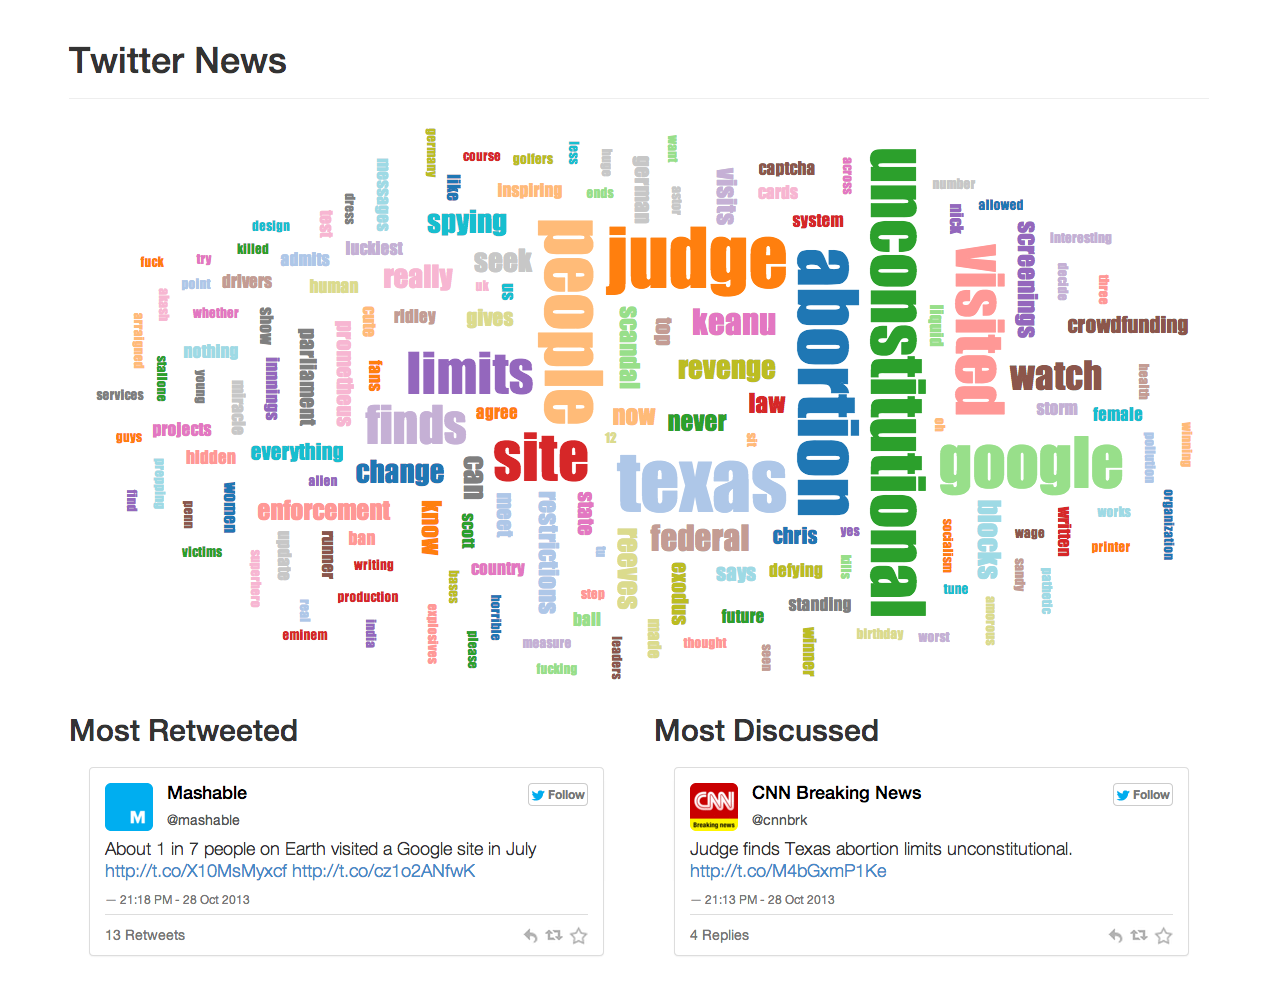
\includegraphics[width=\textwidth]{twitter_news.png}
\caption{Die TwitterNews-Anwendung}
\label{fig:die_twitternews_anwendung}
\end{figure}

% subsection die_client_seite (end)

% section umsetzung (end)

% chapter anwendung (end)
%!TEX root = thesis.tex

\chapter{Fazit und Ausblick} % (fold)
\label{cha:fazit_und_ausblick}

In diesem abschließenden Kapitel wird ein Fazit aus den in dieser Arbeit vorgestellten Inhalten gezogen.
Anschließend wird ein Ausblick gegeben, was in dieser Arbeit nicht behandelt werden konnte, aber was aufbauend auf dieser oder in ihrem thematischen Umfeld für Vorschungsmöglichkeiten bestehen.

\section{Fazit} % (fold)
\label{sec:fazit}

Ziel dieser Arbeit war es, herauszufinden, wie mit Play Web-Anwendungen für das Real-Time-Web entwickelt werden können.
Dazu wurde in den Grundlagen erklärt, wie eine einfache statische Web-Anwendung entwickelt wird.
Diese Anwendung wurde mit den Erkenntnissen der Arbeit später um den Real-Time-Aspekt erweitert.
Dies ließ sich mit den Möglichkeiten des Frameworks verhältnismäßig leicht umsetzen.
Der komplizierteste Teil war das Verständnis der Iteratee-Streams und das Wissen um die denen zugrundeliegenden Konzepte, wie Monaden und speziell die \lstinline|Future|-Monade.

Iteratee-Streams bestehen aus den drei Teilen \lstinline|Enumerator|s, \lstinline|Iteratee|s und \lstinline|Enumeratee|s, also den Datenquellen, den Datensenken und den Stream-Transformatoren.
In dieser Arbeit wurde nicht nur gezeigt, wie diese Komponenten angewendet werden, sondern auch, wie eigene \lstinline|Enumerator|s, \lstinline|Iteratee|s und \lstinline|Enumeratee|s erstellt werden können.
Dieser Blick auf die Implementierungsebene ermöglicht aus Sicht des Autors ein wesentlich umfassenderes Verständnis von Plays Iteratee-Streams.

Plays Implementierung der Iteratee-Streams weicht von der ursprünglichen Implementierung Kiselyovs vor allem in dem Punkt ab, dass sie nicht mit beliebigen Monaden sondern nur mit \lstinline|Future|-Monaden arbeitet.
Der Grund hierfür wird sein, dass Play das Ziel hat, durch reaktive Programmierung ohne zu Blockieren möglichst effizient zu sein, weshalb sich die \lstinline|Future|-Monade anbietet, auch wenn im Gegenzug Flexibilität eingebüßt wird.
Dies ist aus Sicht des Autors vertretbar und hat für ihn beim Arbeiten mit Play keine Probleme dargestellt.

Dass durch diese Streams aber auch komplexere Prozesse als die erste Beispielanwendung implementiert werden können, wurde mit der Twitter News-Anwendung gezeigt.
Dabei wurden mit \lstinline|Iteratee|s Daten von der Twitter-API empfangen und verarbeitet.
Mit verknüpften \lstinline|Enumeratee|s wurden weitere Tweets heruntergeladen und zwischengespeichert.
Erst nach vollständiger Verarbeitung wurden diese Daten wieder als \lstinline|Enumerator|s der Außenwelt zur Verfügung gestellt und deren Elemente an die verbundenen Clients gesendet.
Insgesamt bilden die von Play zur Verfügung gestellten Werkzeuge aus Sicht des Autors eine solide Grundlage, um Real-Time-Web-Anwendungen in einem reaktiven Stil zu entwickeln.

% section fazit (end)

\section{Ausblick} % (fold)
\label{sec:ausblick}

In dieser Arbeit wurde das Hauptaugenmerk auf Play, also die Server-Seite gerichtet und die Client-Seite nur oberflächlich behandelt.
Durch Einsatz eines passenden JavaScript-Frameworks könnte der client-seitige Code wesentlich besser strukturiert werden, wodurch sich Anwendungen mit einer komplexeren Client-Seite besser umsetzen ließen.
Eine weitere Arbeit könnte sich auf die Programmierung der Browser-Seite mit z.~B. AngularJS \cite[vgl.][]{angular_js} oder \mbox{Ember.js} \cite[vgl.][]{ember_js} konzentrieren, die mit einem in Play geschriebenen Server-Backend kommuniziert. % \mbox to prevent line break

Des Weiteren hat sich diese Arbeit fast ausschließlich mit den reaktiven Möglichkeiten des Play-Frameworks beschäftigt, weil diese für die Entwicklung von Real-Time-Web-Anwendungen nötig sind.
Auf viele andere Teile von Play wurde gar nicht oder nur wenig eingegangen, weil dies den Rahmen dieser Arbeit gesprengt hätte.
So wurde beispielsweise das Arbeiten mit Datenbanken komplett ignoriert und für Controller wurde nur die Programmierung einfacher Actions erklärt.
Auch in dieser Richtung gibt es also weitere Möglichkeiten für Forschungen.

Play legt großen Wert auf reaktive Programmierung.
Dieser Trend reduziert sich allerdings nicht alleine auf Play, sondern wird auch von Martin Odersky, dem Begründer von Scala, in einer Online-Vorlesung \cite[vgl.][]{principles_of_reactive_programming} gelehrt.
Die in dieser Arbeit vorgestellten reaktiven Konzepte sind nur ein kleiner Teil der Dinge, die reaktive Programmierung ausmachen.
Jonas Bonér, der Mitarbeiter bei Typesafe ist, hat unter Mitwirkung anderer Persönlichkeiten der Scala-Community das Reactive Manifesto \cite[vgl.][]{reactive_manifesto} veröffentlicht, in dem die Kernpunkte reaktiver Programmierung beschrieben werden.
Dieses Thema bietet genügend Stoff für eine weiterführende Arbeit darüber.

% section ausblick (end)

% chapter fazit_und_ausblick (end)




%%%%

%% appendix if used
%%\appendix
%%\typeout{===== File: appendix}
%%\include{appendix}

% bibliography and other stuff
\backmatter

\typeout{===== Section: literature}
%% read the documentation for customizing the style
\bibliographystyle{dinat}
\bibliography{thesis}

\typeout{===== Section: nomenclature}
%% uncomment if a TOC entry is needed
% \addcontentsline{toc}{chapter}{Glossar} % done via \usepackage[toc]{glossaries}
\renewcommand{\nomname}{Glossar}

% s/Glossary/Glossar/
% \renewcommand*{\glossaryname}{Glossar}
% \deftranslation{Glossary}{Glossar}
\renewcommand*{\acronymname}{Glossar}
\deftranslation{Acronyms}{Glossar}

\printglossaries
\clearpage
\markboth{\nomname}{\nomname} %% see nomencl doc, page 9, section 4.1
\printnomenclature

%% index
\typeout{===== Section: index}
\printindex

\HAWasurency

\end{document}
